%! TEX root = ../../main_netxpto.tex

	\subsection{Simulation Analysis}
	The M-QAM transmission system is a set of blocks that simulate the
	modulation, transmission and demodulation of an optical signal using M-QAM
	modulation. It is composed of several complex blocks: a transmitter, a
	receiver, a noise source, an addition block, a sink and a block that performs a Bit Error Rate (BER) measurement.
	The schematic representation of the system is presented in
	Figures~\ref{fig:sim_systemDiagram} to~\ref{fig:sim_rxDiagram}. The 
	simulation currently implements a QPSK system (M=4).

	\subsubsection{Functional description}
	A complete description of the M-QAM transmitter and M-QAM homodyne receiver
	blocks can be found in the \textit{Library} chapter of this document as well as
	a detailed description of the independent blocks that compose these blocks.
	The M-QAM transmitter generates one or two optical signals by encoding a binary
	string using M-QAM modulation. It also outputs a binary signal that is used to
	perform the BER measurement. The optical signal is then sent through a fiber 
	block, which attenuates it, simulating transmission over a given distance. 
	Aftwerwards, as EDFA block is present to be used as an optical preamplifier. 
	The amplified optical signal, with added ASE noise, is then sent to the 
	homodyne receiver.

	
	The homodyne receiver requires two optical inputs: one of the signal itself, 
	and another from a local oscillator perform the signal demodulation. It 
	receives, processes and decodes the received signal and afterwards outputs 
	the reconstructed bitstream. 
	This signal is compared to the binary signal generated by the
	transmitter in order to estimate the Bit Error Rate (BER).
	The files used are summarized in tables~\ref{tab:sources} and~\ref{tab:headers}.
	All the blocks and sub-blocks used are included in the tables.

	\begin{figure}[h]
		\centering
		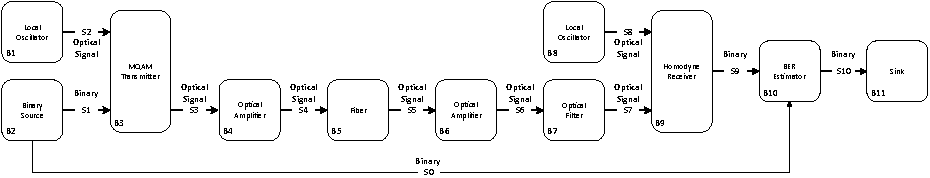
\includegraphics[width=1\textwidth]
			{./sdf/m_qam_system/figures/simulations/blockDiagrams/simulation_mqam}
		\caption{Top-Layer Schematic representation of the simulated MQAM 
		system.}\label{fig:sim_systemDiagram}
	\end{figure}
	\begin{figure}[]
		\centering
		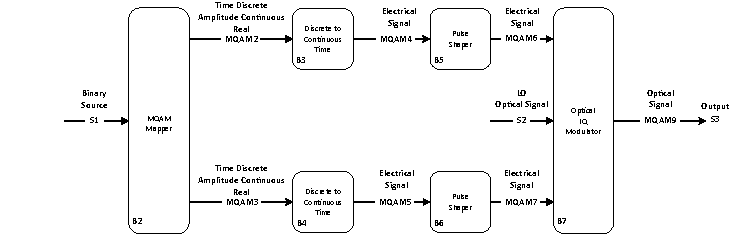
\includegraphics[width=1\textwidth]
			{./sdf/m_qam_system/figures/simulations/blockDiagrams/simulation_tx}
		\caption{Schematic representation of the MQAM Transmitter 
		block.}\label{fig:sim_txDiagram}
	\end{figure}
	\begin{figure}[]
		\centering
		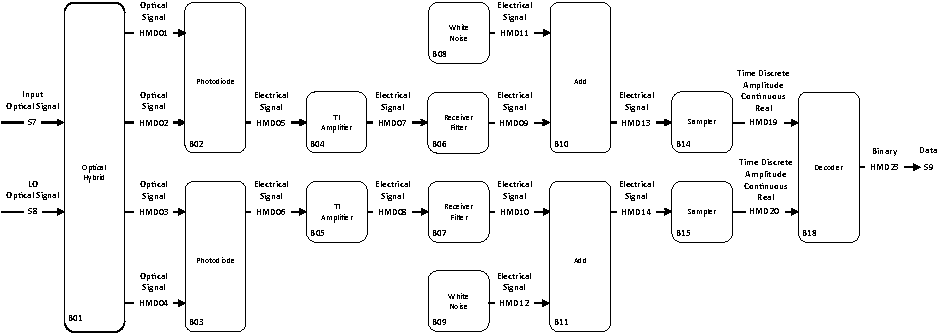
\includegraphics[width=1\textwidth]
			{./sdf/m_qam_system/figures/simulations/blockDiagrams/simulation_rx}
		\caption{Simplified schematic representation of the Homodyne Receiver 
block.}\label{fig:simulation_rx}
	\end{figure}

	\begin{figure}[]
	\centering
	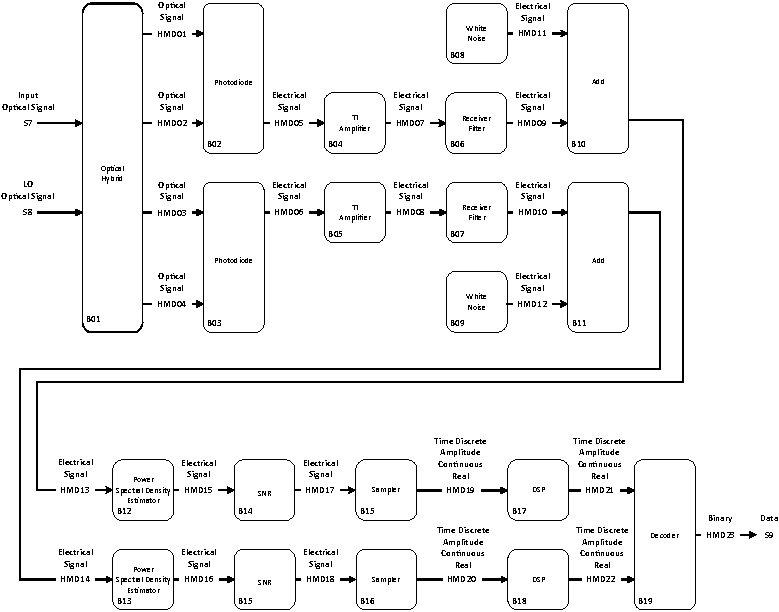
\includegraphics[width=0.9\textwidth]
	{./sdf/m_qam_system/figures/simulations/blockDiagrams/simulation_rx_wSNRAndPSD}
	\caption{Schematic representation of the Homodyne Receiver block, with the 
	DSP block (currently not implemented) and 
	two optional blocks for measuring the SNR and power spectral 
	density.}\label{fig:sim_rxDiagram}
\end{figure}


%\pagebreak
	\clearpage

	\subsubsection{Required files}\label{sec:requiredFilesMQAM}
	\begin{longtable}[h]{|l|l|l|}
		\hline
		\multicolumn{3}{|c|}{ \textbf{Source Files} } \\
		\hline
		\textbf{File}                                     & \textbf{Comments} & \textbf{Status} \\ \hline
		add\_20190215.cpp                                 &                   & 
		\checkmark \\ \hline
		binary\_source\_20190215.cpp                      &                   & 
		\checkmark \\ \hline
		bit\_error\_rate\_20190215.cpp                    &                   & 
		\checkmark \\ \hline
		decoder\_20190215.cpp                             &                   & 
		\checkmark \\ \hline
		discrete\_to\_continuous\_time\_20190215.cpp      &                   & 
		\checkmark \\ \hline
		electrical\_filter\_20190215.h                    &                   & 
		\checkmark \\ \hline
		edfa\_20190215.cpp                                          
		&                   & 
		\checkmark \\ \hline
		fft\_20180208.cpp                                 &                   & \checkmark \\ \hline
		fiber\_20190215.cpp                                         
		&                   & 
		\checkmark \\ \hline
		homodyne\_receiver\_withoutLO\_20190215.cpp                 & 
		$^{1}$            & 
		\checkmark \\ \hline
		ideal\_amplififer\_20190215.cpp                   &                   & 
		\checkmark \\ \hline
		iq\_modulator\_20190215.cpp                       &                   & 
		\checkmark \\ \hline
		local\_oscillator\_20190215.cpp                   &                   & 
		\checkmark \\ \hline
		m\_qam\_mapper\_20190215.cpp                      &                   & 
		\checkmark \\ \hline
		m\_qam\_system\_sdf.cpp                           & $^{2}$            & \checkmark \\ \hline
		m\_qam\_transmitter\_20190215.cpp                 &                   & 
		\checkmark \\ \hline
		netxpto\_20190215.cpp                             & $^{2}$            & 
		\checkmark \\ \hline
		optical\_hybrid\_20190215.cpp                     &                   & 
		\checkmark \\ \hline
		photodiode\_old\_20190215.cpp                     &                   & 
		\checkmark \\ \hline
		power\_spectral\_density\_estimator\_20190215.cpp &                   & 
		\checkmark \\\hline
		pulse\_shaper\_20190215.cpp                       &                   & 
		\checkmark \\ \hline
		sampler\_20190215.cpp                             &                   & 
		\checkmark \\ \hline
		sink\_20190215.cpp                                &                   & 
		\checkmark \\ \hline
		snr\_estimator\_20190215.cpp                      &                   & 
		\checkmark \\\hline
		super\_block\_interface\_20190215.cpp             & $^{2}$            & 
		\checkmark \\ \hline
		white\_noise\_20190215.cpp                        &                   & 
		\checkmark \\ \hline
		window\_20180704.cpp                              &                   & 
		\checkmark \\\hline
		\caption{$^1$ The library entry is under a different name, \textit{m\_qam\_receiver};\\
			$^2$ No library entry as it is a main or general purpose file, not a
		specific block.\label{tab:sources}}\\
	\end{longtable}

	\begin{longtable}[h]{|l|l|l|}
		\hline
		\multicolumn{3}{|c|}{ \textbf{Header Files} } \\
		\hline
		\textbf{File}                                   & \textbf{Comments} & \textbf{Status} \\ \hline
		add\_20190215.h                                 &                   & 
		\checkmark \\ \hline
		binary\_source\_20190215.h                     &                   & 
		\checkmark \\ \hline
		bit\_error\_rate\_20190215.h                    &                   & 
		\checkmark \\ \hline
		decoder\_20190215.h                             &                   & 
		\checkmark \\ \hline
		discrete\_to\_continuous\_time\_20190215.h      &                   & 
		\checkmark \\ \hline
		electrical\_filter\_20190215.h                  &                   & 
		\checkmark \\\hline
		edfa\_20190215.h                                          
		&                   & 
		\checkmark \\ \hline
		fft\_20180208.h                                 &                   & \checkmark \\\hline
		fiber\_20190215.h                                         
		&                   & 
		\checkmark \\ \hline
		homodyne\_receiver\_withoutLO\_20190215.h                 & 
		$^{1}$            & 
		\checkmark \\ \hline
		ideal\_amplifier\_20190215.h                    &                   & 
		\checkmark \\ \hline
		iq\_modulator\_20190215.h                       &                   & 
		\checkmark \\ \hline
		local\_oscillator\_20190215.h                   &                   & 
		\checkmark \\ \hline
		m\_qam\_mapper\_20190215.h                      &                   & 
		\checkmark \\ \hline
		m\_qam\_transmitter\_20190215.h                 &                   & 
		\checkmark \\ \hline
		netxpto\_20190215.h                             & $^2$              & 
		\checkmark \\ \hline
		optical\_hybrid\_20190215.h                     &                   & 
		\checkmark \\ \hline
		photodiode\_old\_20190215.h                     &                   & 
		\checkmark \\ \hline
		power\_spectral\_density\_estimator\_20190215.h &                   & 
		\checkmark \\\hline
		pulse\_shaper\_20190215.h                       &                   & 
		\checkmark \\ \hline
		sampler\_20190215.h                             &                   & 
		\checkmark \\ \hline
		sink\_20190215.h                                &                   & 
		\checkmark \\ \hline
		snr\_estimator\_20190215.h                      &                   & 
		\checkmark \\\hline
		super\_block\_interface\_20190215.h             & $^2$              & 
		\checkmark \\ \hline
		white\_noise\_20190215.h                        &                   & 
		\checkmark \\ \hline
		window\_20180704.h                              &                   & 
		\checkmark \\\hline
		\caption{$^1$ The library entry is under a different name, \textit{m\_qam\_receiver}\\
			$^2$ No library entry as it is a main or general purpose file, not a
		specific block. \label{tab:headers}}\\
	\end{longtable}

	\subsubsection{Input Parameters}\label{sec:inputParamsMQAM}

	\begin{longtable}[h]{|c|c|p{5cm}|}
		\caption{Input parameters}\label{table:in_par}\\\hline

		\textbf{Parameter} & \textbf{Type} & \textbf{Description}     \\ \hline

		numberOfBitsGenerated         & t\_integer
																	& Determines the number of bits to be generated by the
																	binary source\\ \hline
		samplingRate                  & double
																	& The simulation sampling rate \\\hline
		symbolRate                    & double
																	& The symbol rate of the main signal \\\hline
		samplesPerSymbol              & t\_integer
																	& Number of samples per symbol. Defined from
																	the samplingRate and symbolRate.    \\ \hline
		symbolPeriod                  & double
																	& Period of the main signal \\\hline
		bitPeriod                     & double
																	& Periodicity of bits in the main signal \\\hline
		prbsPatternLength             & int
																	& Determines the length of the pseudorandom
																	sequence Pattern (used only when the binary
																	source is operated in \textit{PseudoRandom}
																	mode)     \\ \hline
		bitPeriod                     & t\_real
																	& Temporal interval occupied by one bit     \\ \hline
		rollOffFactor\_shp            & t\_real
																	& Roll-off factor of the pulse shaper filter     \\ \hline
		rollOffFactor\_out            & t\_real
																	& Roll-off factor of the output filter     \\ \hline
		shaperFilter                  & enum
																	& Type of filter used in Pulse Shaper     \\ \hline
		outputFilter                  & enum
																	& Type of filter used in output filter     \\ \hline
		seedType                      & enum
																	& Method of seeding noise generators     \\ \hline
		seedArray                     & array<int,2>
																	& Seeds to initialize noise generators     \\ \hline
		signalOutputPower\_dBm        & t\_real
																	& Determines the power of the output optical
																	signal in dBm   \\ \hline
		numberOfBitsReceived          & int
																	&   Determines when the simulation should
																	stop. If $-1$ then it only stops when there is
																	no more bits to be sent   \\ \hline
		symbolPeriod                  & double
																	& Calculated from symbolRate     \\ \hline
		fiberLength\_m                 & t\_real & Optical fiber length \\\hline
		attentuationCoefficient       & t\_real & Optical fiber attenuation 
		coefficient 
		 \\\hline
		dispersionCoefficient         & t\_real & Optical fiber dispersion 
		coefficient \\\hline
		opticalGain\_dB               & t\_real & Optical gain of the EDFA \\\hline
		noiseFigure                   & t\_real & Noise figure of the EDFA \\\hline
		localOscillatorPower\_dBm     & t\_real
																	& Power of the local oscillator     \\ \hline
		localOscillatorPhase          & t\_real
																	& Phase of the local Oscillator \\\hline
		responsivity                  & t\_real
																	& Responsivity of the photodiodes (1
																	corresponds to having all optical power
																	transformed into electrical current)     \\
																	\hline
		amplification                 & t\_real
																	& Amplification provided by the ideal amplifier     \\ \hline
		thermalNoiseSpectralDensity   & t\_real
																	& Noise spectral density added after the electrical filter \\\hline
		amplifierNoiseSpectralDensity & t\_real
																	& Electrical noise spectral density added before the
																	electrical filter \\\hline
		elFilterType                  & enum
																	& Type of the electrical filter: generated low
																	pass or defined by coefficients \\\hline
		elFilterOrder                 & enum
																	& Order of the electrical filter \\\hline
		impulseResponseArr            & t\_real[]
																	& Array of coefficients of the electrical
																	filter. \\\hline
		iqAmplitudeValues             & vector<t\_iqValues>
																	& Determines the constellation used to encode
																	the signal in IQ space \\\hline
		samplesToSkip                 & t\_integer
																	& Number of samples to be skipped by the
																	\textit{sampler} block     \\ \hline
		confidence                    & t\_real
																	& Determines the confidence limits for the BER
																	estimation     \\ \hline
		midReportSize                 & t\_integer
																	&      \\ \hline
		bitSourceMode                 & enum
																	& Mode of generating the bitstream for the
																	signal	\\\hline
		electricalSNRMethod           & enum
																	& Mode for calculating the SNR prior to the
																	matched filter	\\\hline
		filteredSNRMethod             & enum
																	& Mode for calculating the SNR after the
																	matched filter	\\\hline
		SNRignoreSamples              & int
																	& Number of samples to initially ignore when
																	calculating the SNR \\\hline
		SNRsegmentSize                & int
																	& Size of each segment used for estimating the
																	SNR \\\hline
		powerSpectralDensityOverlap   & double
																	& Percentage of the signal to overlap when
																	averaging periodograms in power spectral
																	density estimation \\\hline
		powerSpectralDensitySegment   & int
																	& Size of segment used for calculating each
																	periodogram \\\hline
		powerSpectralDensityInterval  & int
																	& Number of samples to acquire before
																	estimating the power spectral density \\\hline
		bufferLength                  & t\_integer
																	& Corresponds to the number of samples that
																	can be processed in each run of the system
																	\\ \hline
	\end{longtable}

	\subsubsection{Output Files}\label{sec:outputFilesMQAM}

	\begin{longtable}[h]{|c|p{5cm}|}
		\caption{Output Files}\label{table:out_files}\\\hline

		\textbf{Files} & \textbf{Description}     \\ \hline
		\textit{Signal.sgn}				& Files with corresponding signal data generated
			in the simulation. \\\hline
		BER.txt                   & Results from bit\_error\_rate block. \\ \hline
		log.txt                   & Log file from simulation. \\ \hline
		params.txt                & Input parameter list. \\ \hline
		PowerSpectralDensity.txt  & Power spectral density estimate from optical
			signal. \\ \hline
		PowerSpectralDensity2.txt & Power spectral density estimate from electrical
			signal. \\ \hline
		SNR.txt                   & SNR estimate before matched filter. \\ \hline
		SNRFiltered.txt           & SNR estimate after matched filter.	\\ \hline
		impulse\_response.imp     & Impulse response from electrical filter. \\ \hline
		out\_filter.imp           & Impulse response from matched filter. \\ \hline
		pulse\_shaper.imp         & Pulse shaper impulse response. \\ \hline
	\end{longtable}

\subsubsection{Simulation results - ISI}\label{sec:simRes_ISI}

	In this section we will explore the signals generated during the simulation.
	The general scheme of the simulation is shown in
	Figures~\ref{fig:sim_systemDiagram}, ~\ref{fig:sim_txDiagram}
	and~\ref{fig:sim_rxDiagram}. Every signal generated during the simulation 
	is
	identified in those diagrams.
	
	We will start by analyzing the intersymbol interference (ISI) in the signals 
	generated on the simulation. For this purpose, we will turn of all noise 
	sources. We will be using 
	root-raised cosines at the pulse shaper (\textit{B5} and \textit{B6} on MQAM 
	transmitter) and 
	at the matched filter (\textit{B18} and \textit{B19} at the homodyne 
	receiver). With this 
	configuration, we should obtain a perfect copy of the transmitted 
	constellation, affected only by a scaling factor (which could be removed by 
	adjusting the \textit{amplification} parameter).

	The parameters used to obtain the plots and eye diagrams
	in this section are displayed in Table~\ref{tab:noNoiseSimParams}.

	\begin{longtable}[h]{|l|l|l|}
		\caption{Simulation parameters\label{tab:noNoiseSimParams}}\\\hline
		\textbf{Parameter}            & \textbf{Value}       &\textbf{Units}\\\hline
		numberOfBitsGenerated         & $100 \times 10^3$    & \\\hline
		samplingRate                  & $64 \times 10^9$     & Hz \\\hline
		symbolRate                    & $4 \times 10^9$      & Bd \\\hline
		samplesPerSymbol              & 16                   & \\\hline
		symbolPeriod                  & $250\times 10^{-12}$ & s\\\hline
		bitPeriod                     & $125\times 10^{-12}$ & s\\\hline
		signalOutputPower\_dBm        & -10                  & dBm\\\hline
		localOscillatorPower\_dBm     & 0                    & dBm\\\hline
		localOscillatorPhase          & 0                    & rad\\\hline
		nBw                           & $18\times10^9$       & Hz\\\hline
		amplification                 & 3162.28              & \\\hline
		responsivity                  & 1                    & A/W\\\hline
		outputFilter                  & RootRaisedCosine     & \\\hline
		shaperFilter                  & RootRaisedCosine     & \\\hline
		rollOffFactor\_out            & 0.9                  & \\\hline
		rollOffFactor\_shp            & 0.9                  & \\\hline
		seedType                      & RandomDevice         & \\\hline
		numberOfBitsReceived          & -1                   & \\\hline
		elFilterType                  & Defined              & \\\hline
		elFilterOrder                 & 20                   & \\\hline
		opticalGain\_dB               & 0                    & dB \\\hline
		noiseFigure                   & 0                    & dB \\\hline
		preFilterNoiseSpectralDensity & 0                    & W/Hz\\\hline
		elNoiseSpectralDensity        & 0                    & W/Hz\\\hline
		bufferLength                  & 512                  & \\\hline
		bitSourceMode                 & Random               & \\\hline
		confidence                    & 0.95                 & \\\hline
	\end{longtable}


	We will start by showing the signals present in the 
	\textit{m\_qam\_transmitter} block, shown
	in Figure~\ref{fig:sim_txDiagram}. This is the block where the signals are 
	generated and modulated, and remains unaltered for all cases shown here. 
	Therefore, to avoid repetition, these signals will only be shown here, as 
	their properties remain similar for all the other simulation that will be 
	examined further on.

	First, the initial bitstream is generated. This is the pseudorandom array of 
	ones and zeros which will be transmitted, and later compared with the decoded 
	signal.
	
	% Initial bitstream
	\begin{figure}[H]
			\centering
\begin{minipage}{0.45\textwidth}
	\centering
	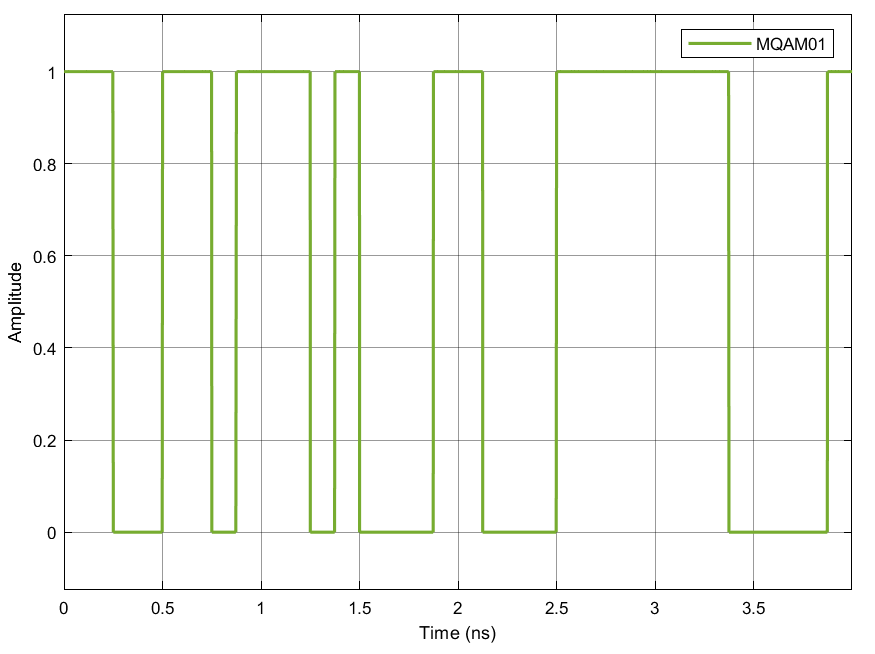
\includegraphics[width=1\textwidth]
	{./sdf/m_qam_system/figures/simulations/01_noISI/MQAM01.pdf}
	\subcaption{}
\end{minipage}
\begin{minipage}{0.4\textwidth}
	\centering
	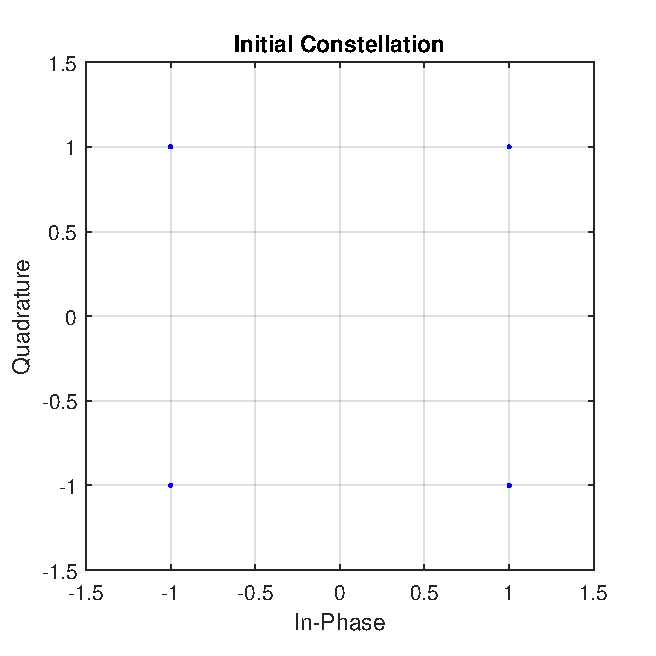
\includegraphics[width=\textwidth]
	{./sdf/m_qam_system/figures/simulations/01_noISI/constStart.pdf}
	\subcaption{}
\end{minipage}
			%			\includegraphics[width=1\textwidth]
			%			{./sdf/m_qam_system/figures/eyes/noNoise/MQAM5.pdf}
			\caption{Eye diagram of initial bitstream MQAM01 (pseudorandom ones and 
			zeros), and respective constellation to be used.}
	\end{figure}

This series of bits needs to be encoded into the corresponding coordinate 
points, according to the chosen constellation and modulation format. As we are 
using a 4 point QAM modulation, these coordinate points are (1,1), (1,-1), 
(-1,-1) and (-1,1). Mapping the bits to these points is done in the 
\textit{MQAM\_mapper} block. This block receives the binary sequence and 
outputs two signals, discrete in time and value. Each bit is alternately coded 
into one of the output signals, according to the chosen constellation. In this 
case, the values are either 1 or -1.
Each signal contains the values ultimately used to modulate either 
the in-phase or quadrature component.

	\begin{figure}[H]
		\centering
		\begin{minipage}{0.45\textwidth}
			\centering
			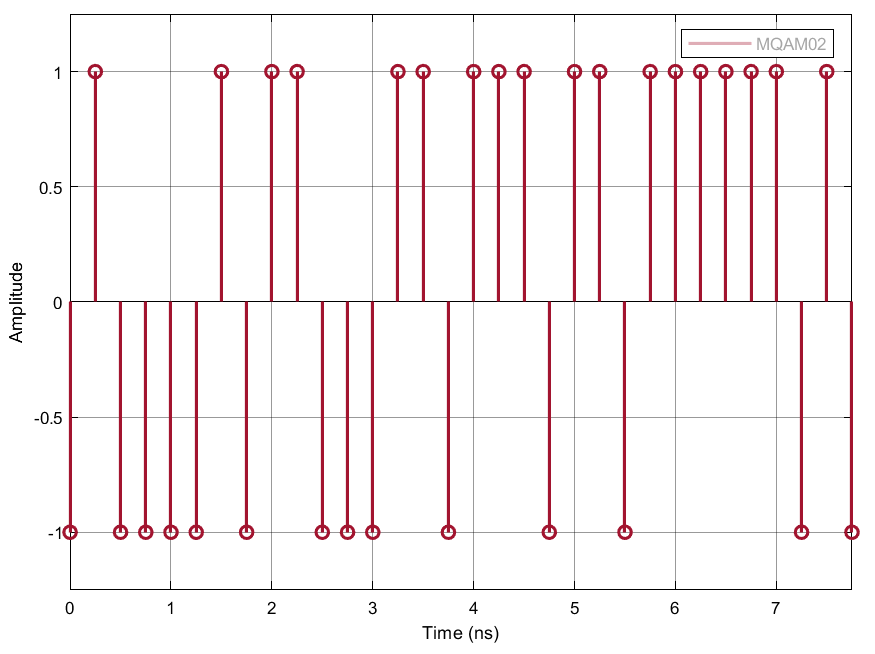
\includegraphics[width=1\textwidth]		
			{./sdf/m_qam_system/figures/simulations/01_noISI/MQAM02.pdf}
			\subcaption{}\label{fig:ISImqam2}
		\end{minipage}
		\begin{minipage}{0.45\textwidth}
			\centering
			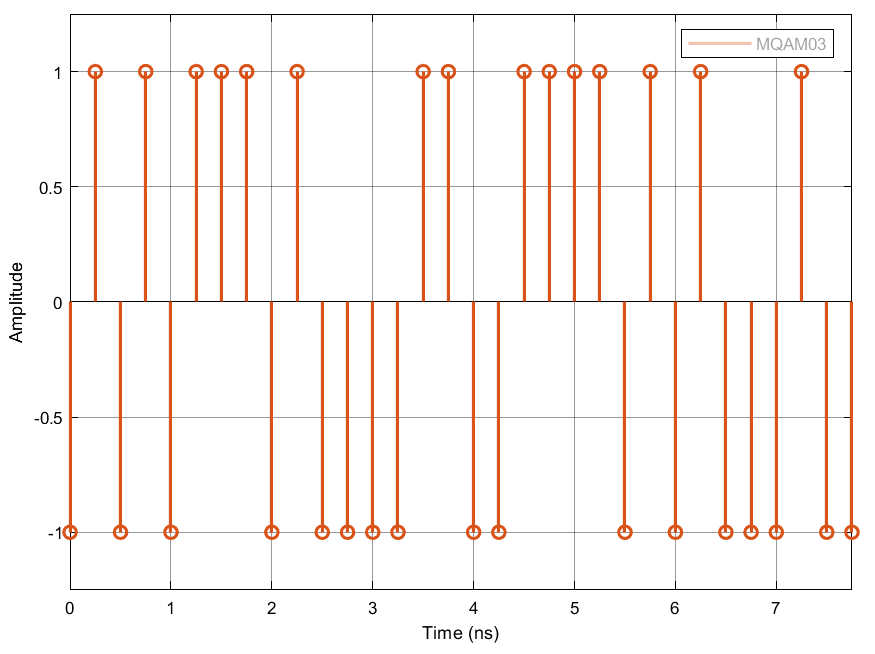
\includegraphics[width=1\textwidth]
			{sdf/m_qam_system/figures/simulations/01_noISI/MQAM03.pdf}
			\subcaption{}\label{fig:ISImqam3}
		\end{minipage}
		\caption{Signals MQAM02~(\subref{fig:ISImqam2}) and 
		MQAM03~(\subref{fig:ISImqam3}), 
		containing the values encoded and distributed to the in-phase and quadrature
		components.}
	\end{figure}

As mentioned before, the signals MQAM02 and MQAM03 are discrete in both value 
and 
time. However, in order to be used for modulating the optical signal, they need 
to 
be continuous in time. Also, they have to be assigned a given continuous 
shape that can be modulated onto the optical signal.

The first of these requirements is fixed with the 
\textit{discrete\_to\_continuous\_time} block. This block takes the discrete 
sequence of values generated on the previous block and outputs an equivalent 
where each value (or symbol) has a proper timing. Therefore, it outputs the 
previous sequence of values, but in an array continuous in time, with each 
value separated by an amount of time 
equal to the desired symbol period.

	\begin{figure}[H]
	\centering
	\begin{minipage}{0.45\textwidth}
		\centering
		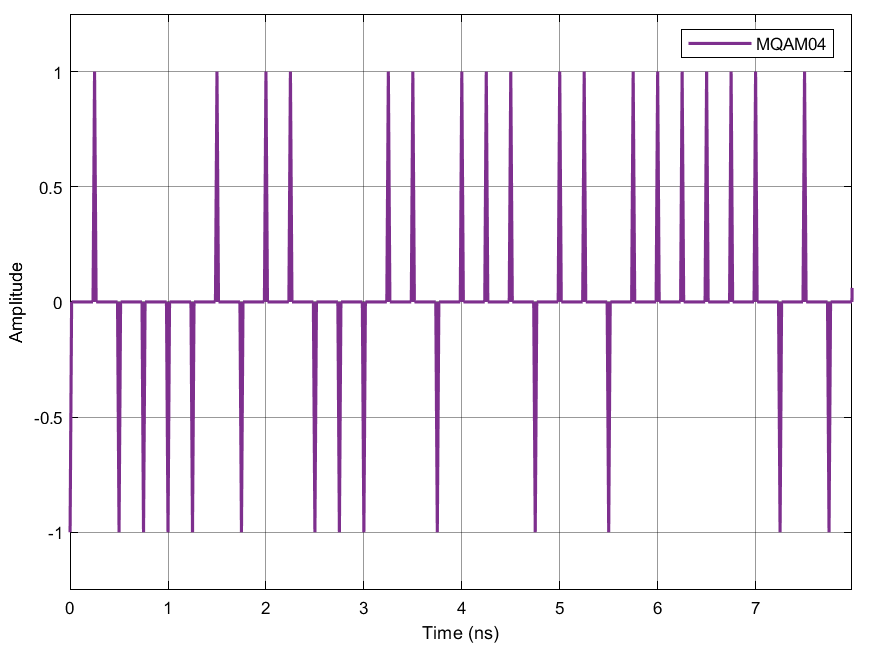
\includegraphics[width=1\textwidth]		
		{./sdf/m_qam_system/figures/simulations/01_noISI/MQAM04.pdf}
		\subcaption{}\label{fig:ISImqam4}
	\end{minipage}
	\begin{minipage}{0.45\textwidth}
		\centering
		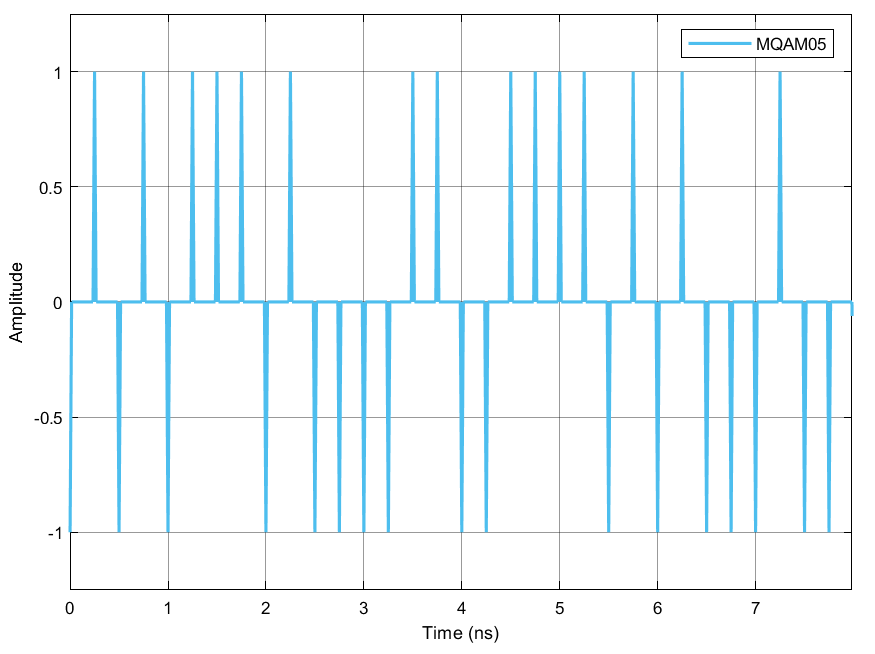
\includegraphics[width=1\textwidth]
		{sdf/m_qam_system/figures/simulations/01_noISI/MQAM05.pdf}
		\subcaption{}\label{fig:ISImqam5}
	\end{minipage}
	\caption{Signals MQAM04~(\subref{fig:ISImqam4}) and 
	MQAM05~(\subref{fig:ISImqam5}), 
		containing the values in a signal with continuous time.}
\end{figure}

	The signals still need to be assigned a continuous shape in order to modulate 
	them into the optical signal. This is done with a pulse shaper, which acts as 
	a 
	FIR filter shaping the discretely-valued sequences of symbols. As mentioned 
	in the beginning of the section, the chosen filter is a root-raised-cosine.

	\begin{figure}[H]
	\centering
	\begin{minipage}{0.45\textwidth}
		\centering
		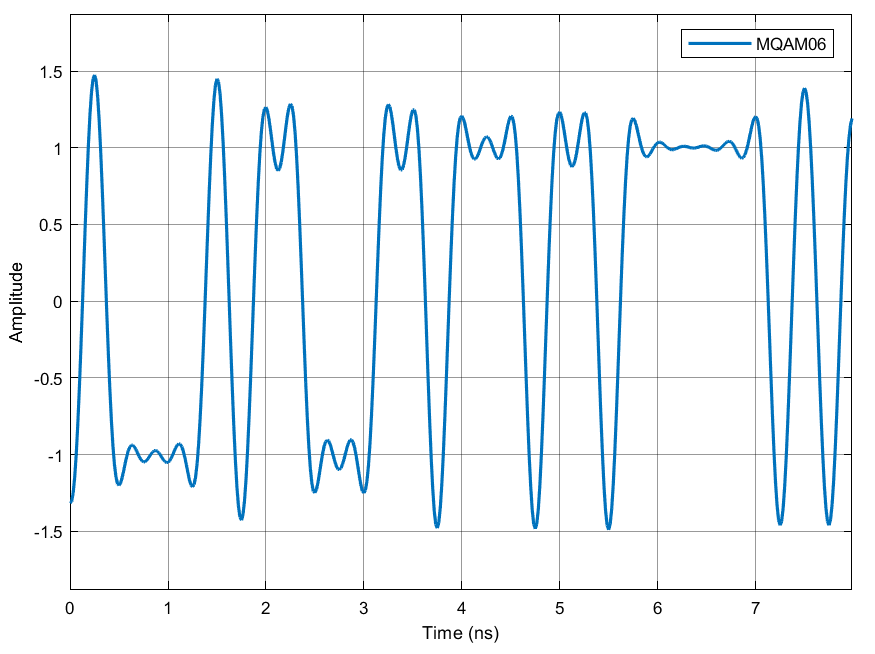
\includegraphics[width=1\textwidth]		
		{./sdf/m_qam_system/figures/simulations/01_noISI/MQAM06.pdf}
		\subcaption{}\label{fig:ISImqam6}
	\end{minipage}
	\begin{minipage}{0.45\textwidth}
		\centering
		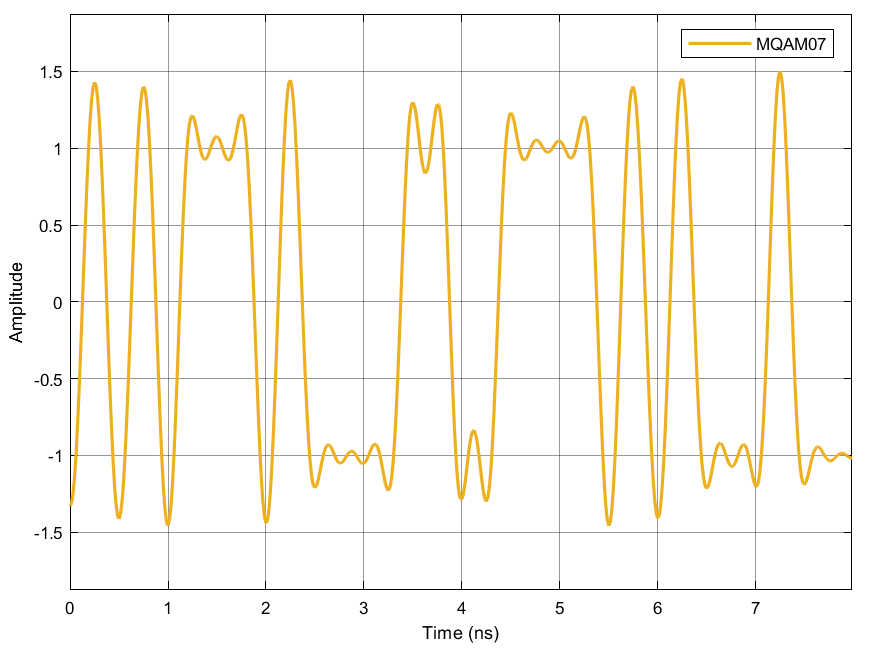
\includegraphics[width=1\textwidth]
		{sdf/m_qam_system/figures/simulations/01_noISI/MQAM07.pdf}
		\subcaption{}\label{fig:ISImqam7}
	\end{minipage}
	\caption{Signals MQAM06~(\subref{fig:ISImqam6}) and 
	MQAM07~(\subref{fig:ISImqam7}), 
		containing the signals to be modulated, already shaped with a 
		root-raised-cosine filter.}
\end{figure}

	\begin{figure}[H]
	\centering
	\begin{minipage}{0.45\textwidth}
		\centering
		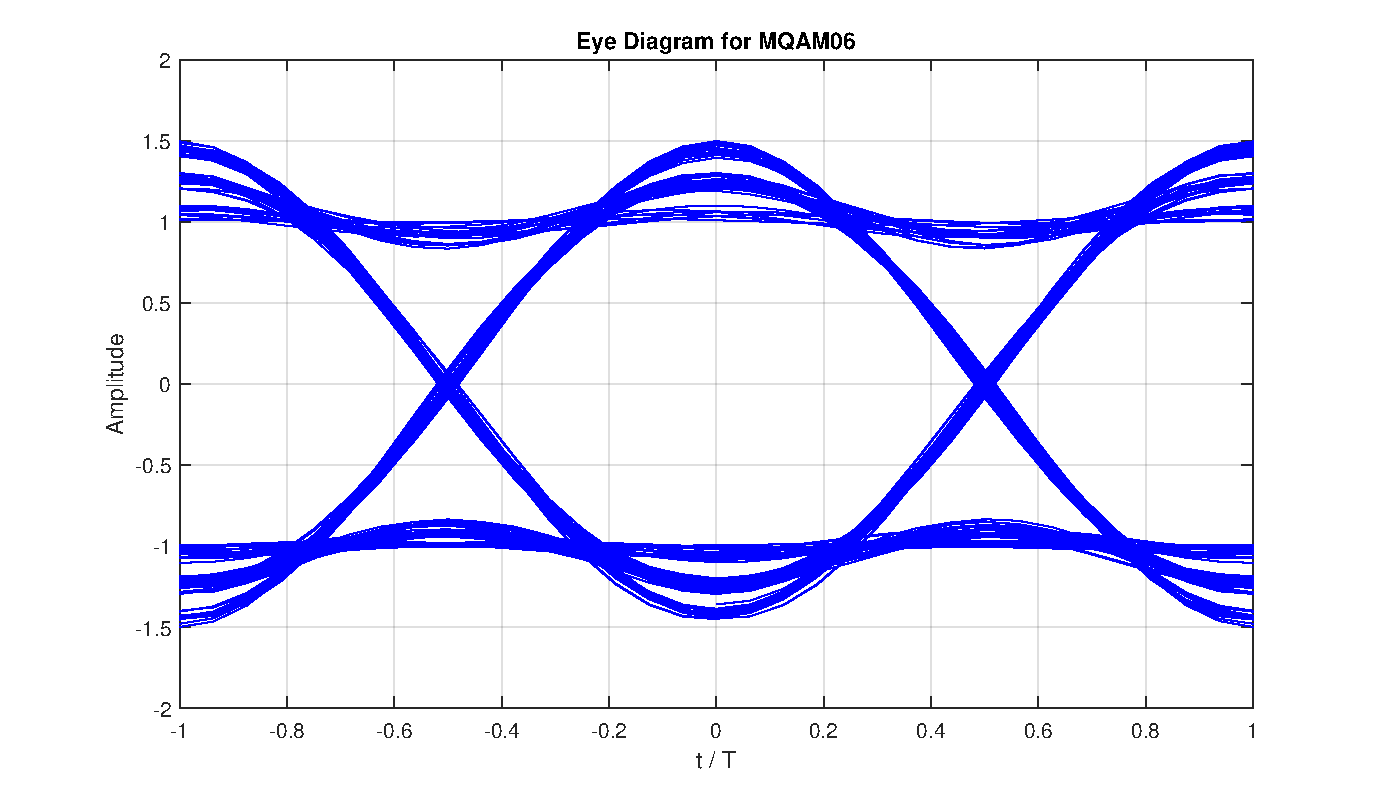
\includegraphics[width=1\textwidth]		
		{./sdf/m_qam_system/figures/simulations/01_noISI/MQAM06_edl.pdf}
		\subcaption{}\label{fig:ISImqam6ed}
	\end{minipage}
	\begin{minipage}{0.45\textwidth}
		\centering
		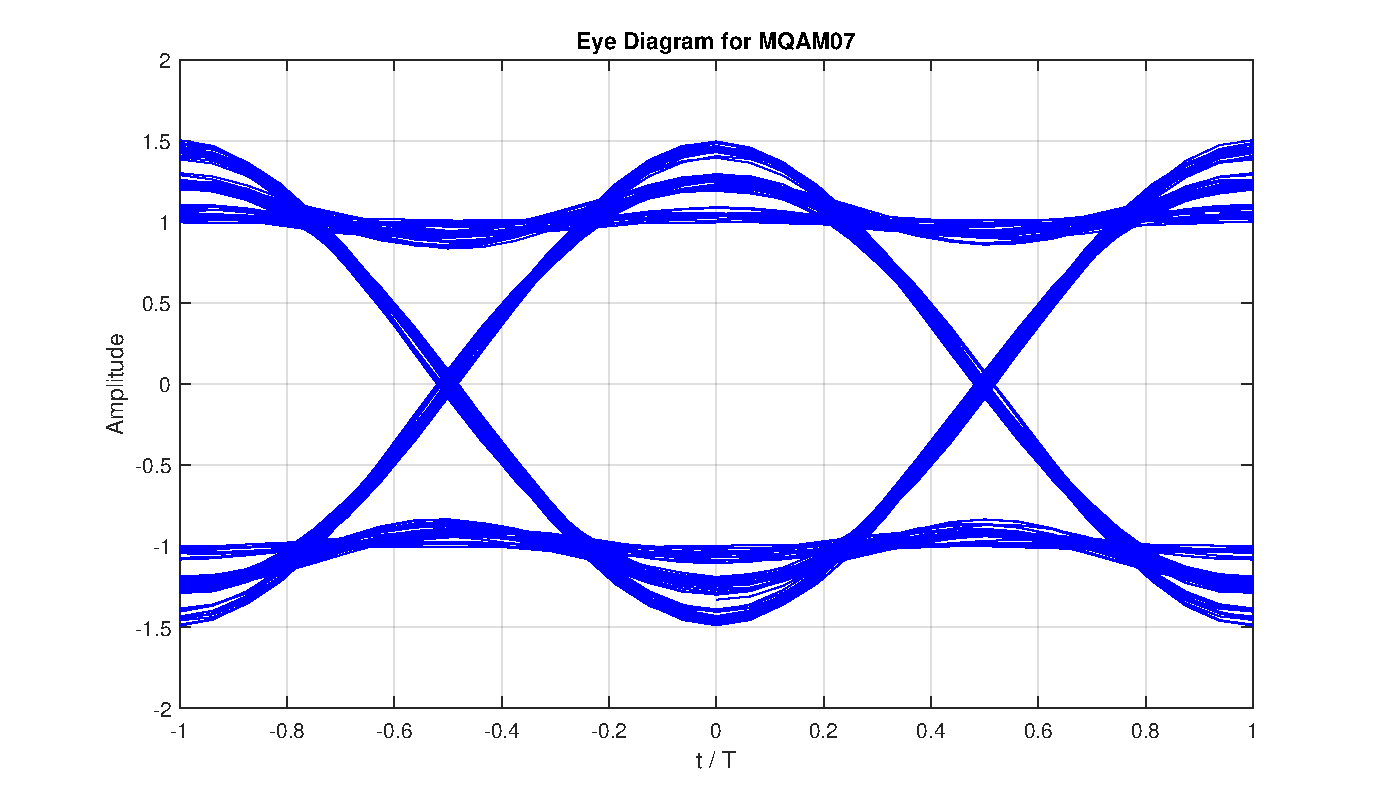
\includegraphics[width=1\textwidth]
		{sdf/m_qam_system/figures/simulations/01_noISI/MQAM07_edl.pdf}
		\subcaption{}\label{fig:ISImqam7ed}
	\end{minipage}
	\caption{Eye diagrams for MQAM06~(\subref{fig:ISImqam6ed}) and 
		MQAM07~(\subref{fig:ISImqam7ed}), shaped with root-raised-cosines.}
\end{figure}

	It can be seen in the eye diagrams that the signal is not free from ISI. 
	However, as mentioned in section~\ref{sec:ISI}, the shaping is done at the 
	transmitter and at the receiver. We shall see further ahead that the signal 
	will be free of ISI at sampling time.

	Being continuous in time and in value, signals MQAM06 and MQAM07 are then 
	ready to be passed on to the 
	\textit{iq\_modulator} block, where they are modulated into an optical 
	signal, and then transmitted.

	\begin{figure}[H]
	\centering
		\centering
		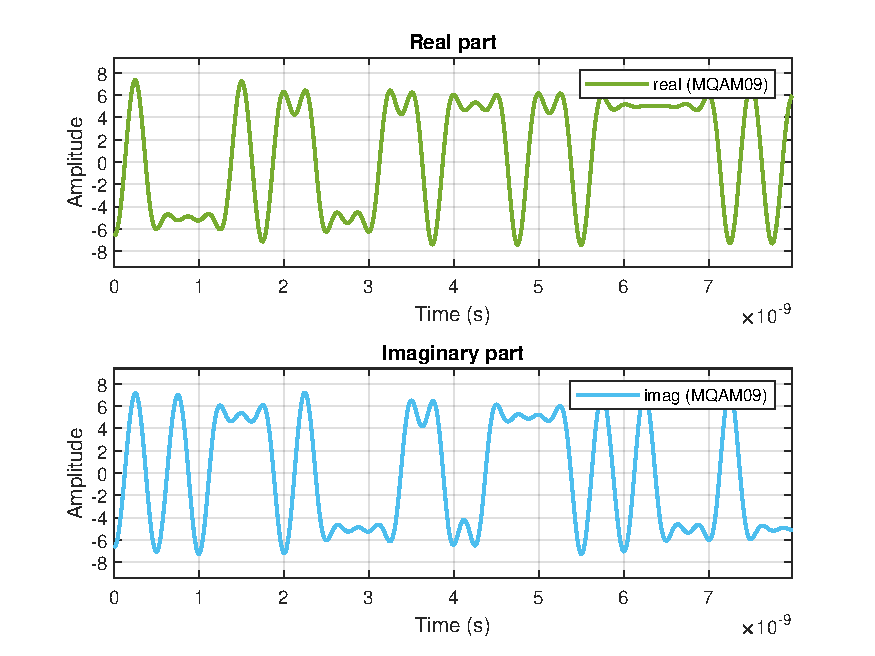
\includegraphics[width=0.7\textwidth]		
		{./sdf/m_qam_system/figures/simulations/01_noISI/MQAM09.pdf}
	\caption{Signal MQAM09, modulated optical signal.}\label{fig:ISImqam9}
\end{figure}

	MQAM01 and MQAM09 are the output signals of the \textit{m\_qam\_transmitter} 
	block. They are equal to the top level signals S0 and S1, respectively.
	Normally the S1 signal is now directed to an \textit{optical\_fiber} block, 
	which is then connected to an \textit{edfa} block. However, in this 
	simulation they are both configured to have no effect, and so we shall not 
	show them here. The optical signal then proceeds to be used as input to the 
	\textit{homodyne\_receiver\_withoutLO} block, along with S4, an optical 
	signal acting as local oscillator.
	
	We shall now explore the process inside the 
	\textit{homodyne\_receiver\_withoutLO} 
	block. The inputs of the block are mixed inside an \textit{optical\_hybrid} 
	block. These outputs are a mix of the transmitted optical signal and the 
	local oscillator, as explained in 
	section~\ref{sec:teorRX}.
	
		% After optical hybrid 1
		\begin{figure}[H]
			\centering
				\centering
				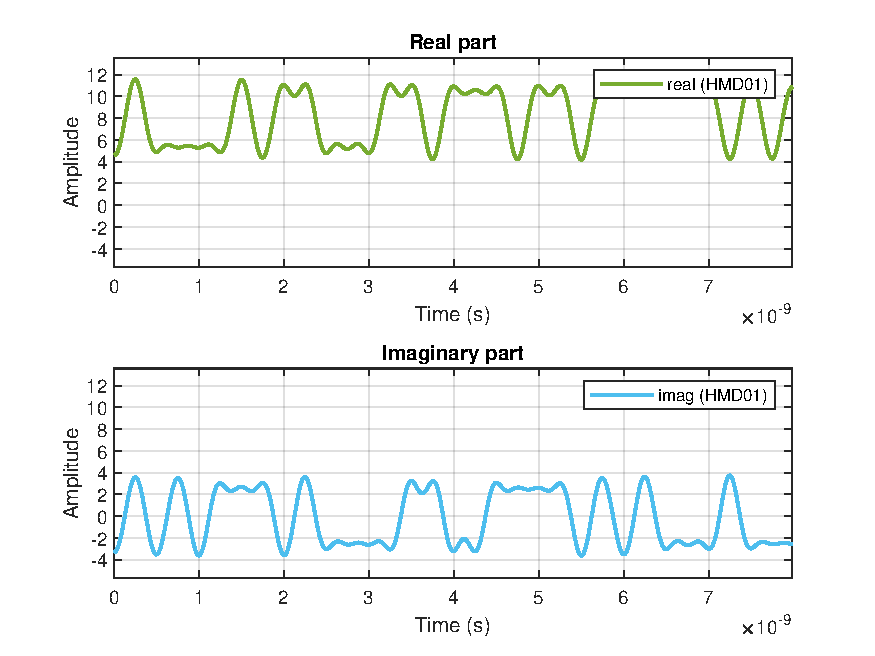
\includegraphics[width=0.7\textwidth]
				{./sdf/m_qam_system/figures/simulations/01_noISI/HMD01.pdf}
						\caption{HMD01, output 1 optical hybrid.}
		\end{figure}
	\begin{figure}[H]
				\centering
				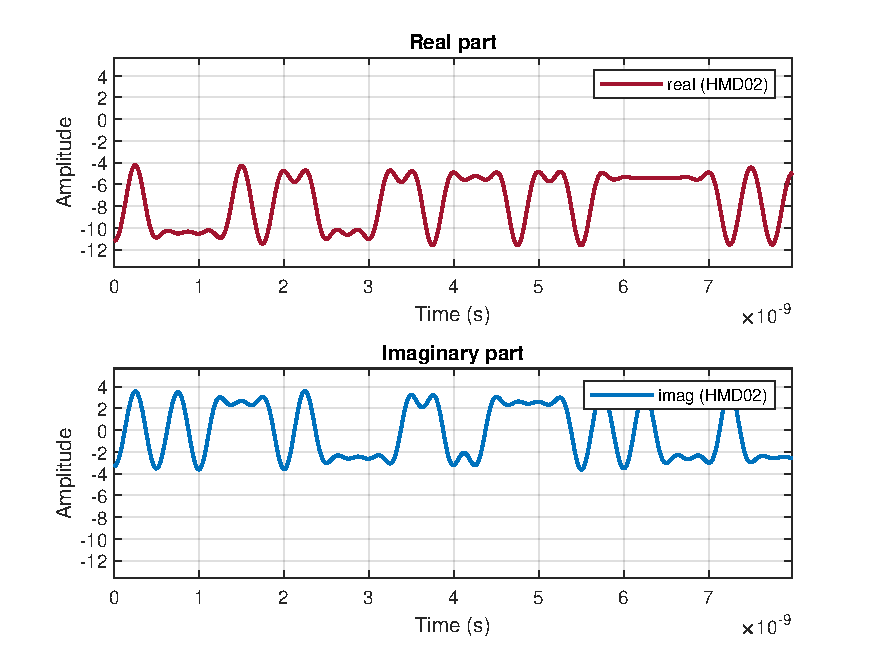
\includegraphics[width=0.7\textwidth]
				{./sdf/m_qam_system/figures/simulations/01_noISI/HMD02.pdf}
		\caption{HMD02, output 2 of the optical hybrid.}
		\end{figure}
	
		\begin{figure}[H]
			\centering
				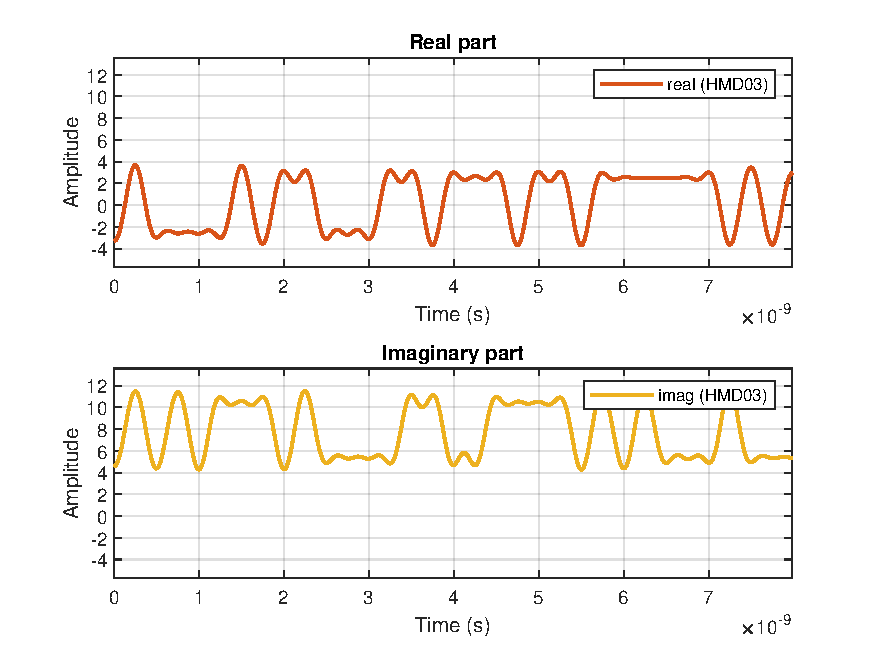
\includegraphics[width=0.7\textwidth]
				{./sdf/m_qam_system/figures/simulations/01_noISI/HMD03.pdf}
		\caption{HMD03, output 3 of the optical hybrid.}
				\end{figure}
	\begin{figure}[H]
				\centering
				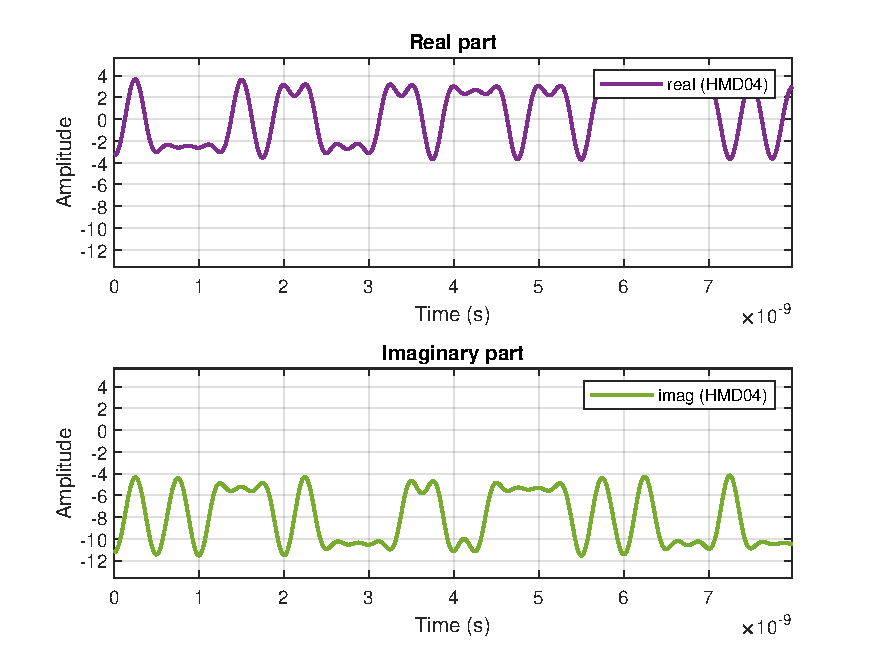
\includegraphics[width=0.7\textwidth]
				{./sdf/m_qam_system/figures/simulations/01_noISI/HMD04.pdf}
		\caption{HMD04, output 4 of the optical hybrid.}
		\end{figure}
		
	These optical signals are then sent in pairs to two \textit{photodiode} 
	blocks, where they are detected (with a \textit{responsivity} defined in the 
	parameters) and 
	subtracted. The output of the photodiode 
	blocks is then directed to the \textit{ti\_amplifier} blocks, which generate 
	the signals shown in Figure~\ref{fig:ISIhmd0708}. The \textit{ti\_amplifier} 
	usually does three things: it adds noise, amplifies the signal and noise, and 
	lastly passes the signal and noise through a filter. However, as there is no 
	noise here and the filter's bandwidth is much larger than the signal 
	bandwidth, the only visible effect is the amplification.

	\begin{figure}[H]
	\centering
	\begin{minipage}{0.45\textwidth}
		\centering
		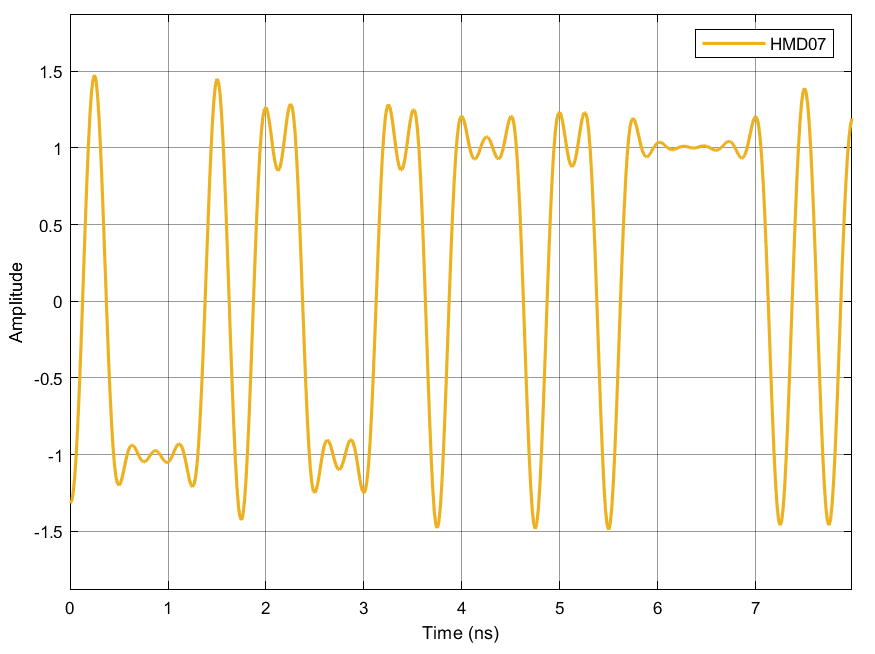
\includegraphics[width=1\textwidth]		
		{./sdf/m_qam_system/figures/simulations/01_noISI/HMD07.pdf}
		\subcaption{}\label{fig:ISIhmd07}
	\end{minipage}
	\begin{minipage}{0.45\textwidth}
		\centering
		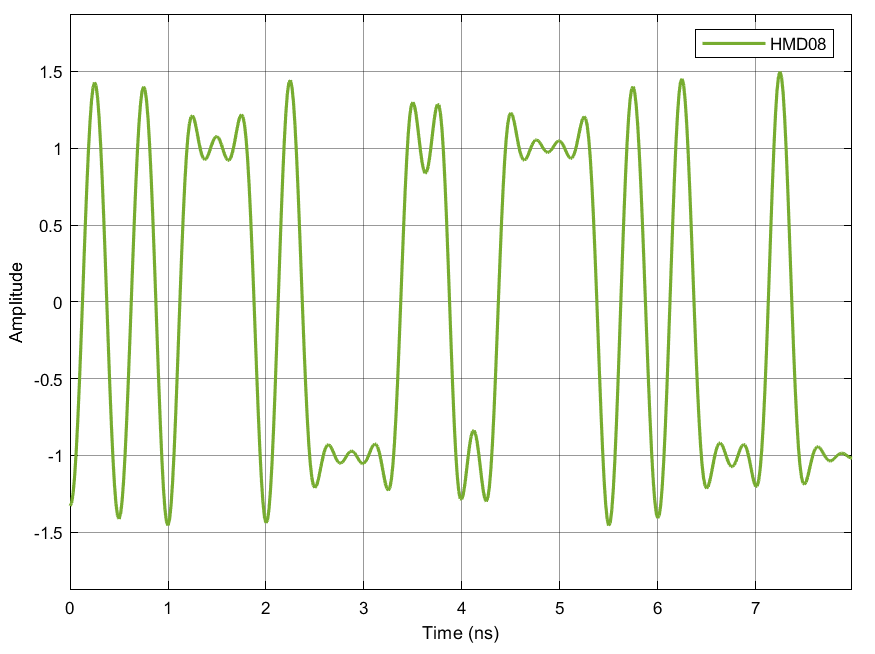
\includegraphics[width=1\textwidth]
		{sdf/m_qam_system/figures/simulations/01_noISI/HMD08.pdf}
		\subcaption{}\label{fig:ISIhmd08}
	\end{minipage}
	\caption{Signals HMD07~(\subref{fig:ISIhmd07}) and 
		HMD08~(\subref{fig:ISIhmd08}), 
		containing the amplified versions of the signals detected at the 
		\textit{photodiode} blocks}\label{fig:ISIhmd0708}
\end{figure}


The next step is the matched filter. Again, as there is no noise, the only 
visible effect is the change in the signal shape. By using another 
root-raised-cosine filter, the signal now follows a raised-cosine shape.

	\begin{figure}[H]
	\centering
	\begin{minipage}{0.45\textwidth}
		\centering
		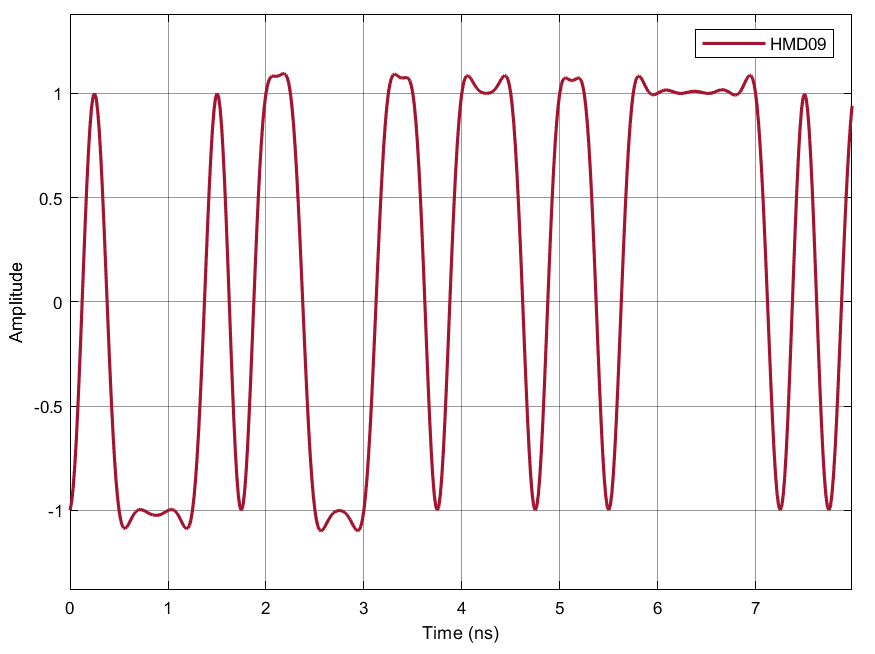
\includegraphics[width=1\textwidth]		
		{./sdf/m_qam_system/figures/simulations/01_noISI/HMD09.pdf}
		\subcaption{}\label{fig:ISIhmd09}
	\end{minipage}
	\begin{minipage}{0.45\textwidth}
		\centering
		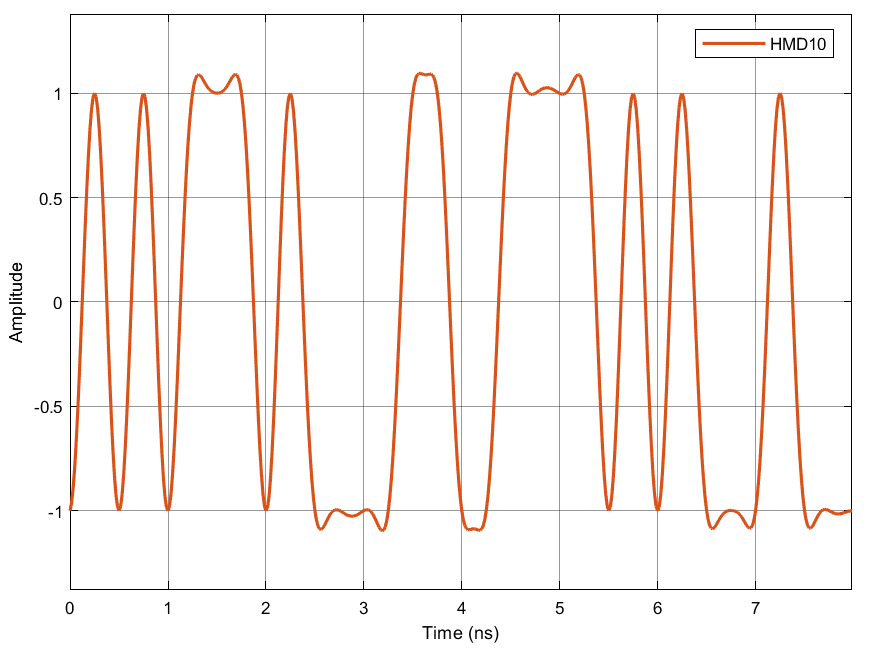
\includegraphics[width=1\textwidth]
		{sdf/m_qam_system/figures/simulations/01_noISI/HMD10.pdf}
		\subcaption{}\label{fig:ISIhmd10}
	\end{minipage}
	\caption{Signals HMD09~(\subref{fig:ISIhmd09}) and 
		HMD10~(\subref{fig:ISIhmd10}), after the root-raised-cosine matched 
		filter.}\label{fig:ISIhmd0910}
\end{figure}


	\begin{figure}[H]
	\centering
	\begin{minipage}{0.45\textwidth}
		\centering
		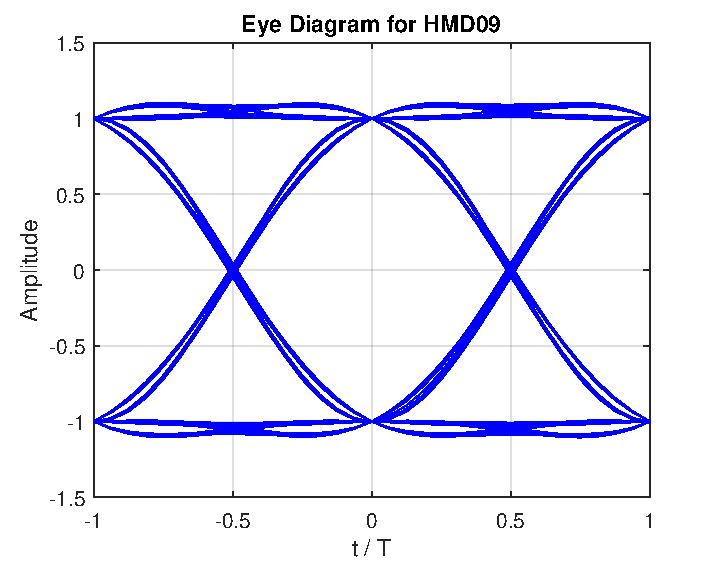
\includegraphics[width=1\textwidth]		
		{./sdf/m_qam_system/figures/simulations/01_noISI/HMD09_ed.pdf}
		\subcaption{}\label{fig:ISIhmd09ed}
	\end{minipage}
	\begin{minipage}{0.45\textwidth}
		\centering
		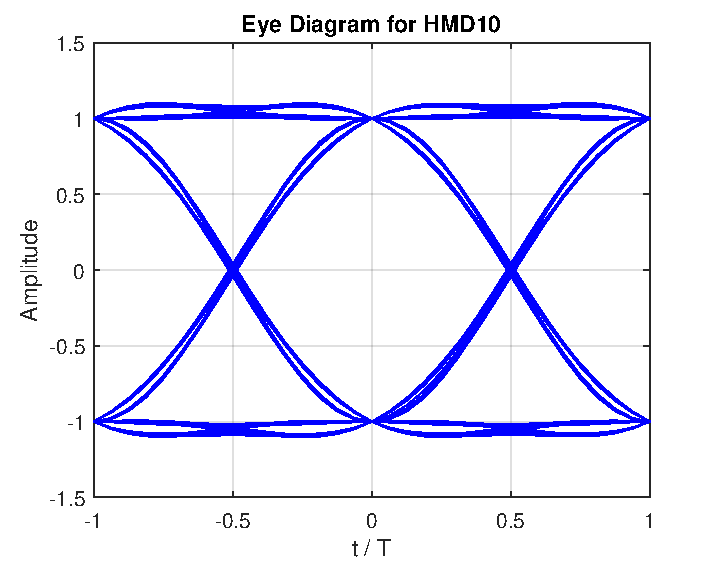
\includegraphics[width=1\textwidth]
		{sdf/m_qam_system/figures/simulations/01_noISI/HMD10_ed.pdf}
		\subcaption{}\label{fig:ISIhmd10ed}
	\end{minipage}
	\caption{Eye diagrams for HMD09~(\subref{fig:ISIhmd09ed}) and 
		HMD10~(\subref{fig:ISIhmd10ed}), after the root-raised-cosine matched 
		filter. They are now following a raised-cosine 
		shape.}\label{fig:ISIhmd0910ed}
\end{figure}

For the purpose of this simulation, no electrical noise is added at the 
receiver. So HMD09 and HMD10 are effectively the signals that will be sampled. 
As can be seen from their 
eye diagrams in Figure~\ref{fig:ISIhmd0910ed}, they suffer from no intersymbol 
interference, having always the same exact value at sampling time. This is then 
sampled and then decoded, transforming the received signal into a bitstream. As 
the reception is perfect, the received bitstream is exactly equal to the 
transmitted one.

	\begin{figure}[H]
	\centering
	\begin{minipage}{0.45\textwidth}
		\centering
		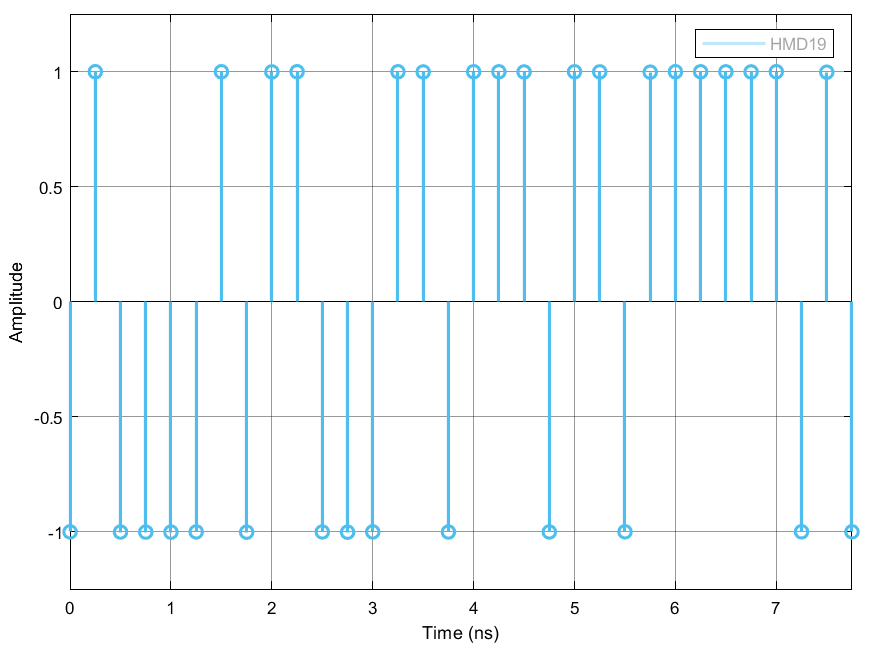
\includegraphics[width=1\textwidth]		
		{./sdf/m_qam_system/figures/simulations/01_noISI/HMD19.pdf}
		\subcaption{}\label{fig:ISIhmd19}
	\end{minipage}
	\begin{minipage}{0.45\textwidth}
		\centering
		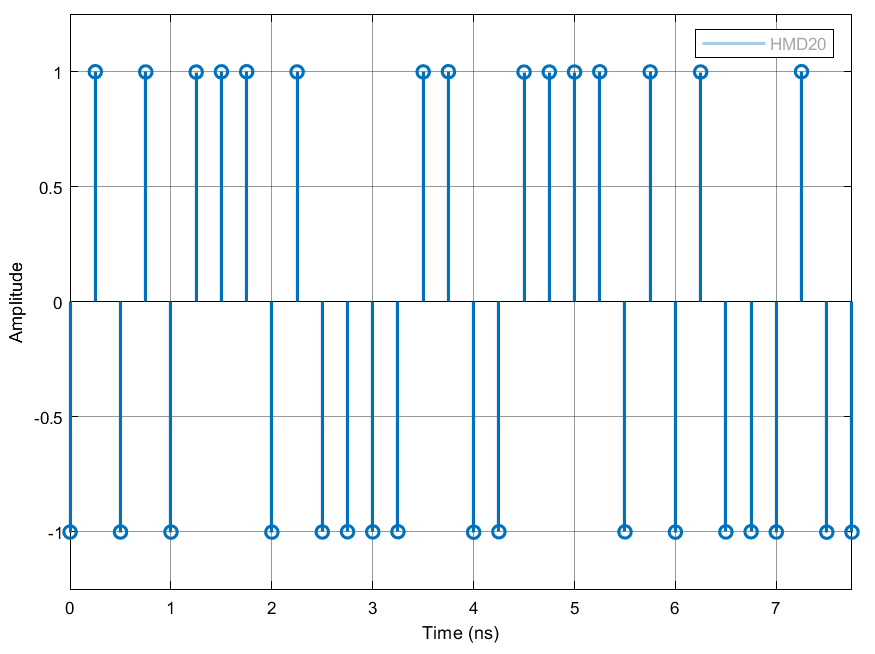
\includegraphics[width=1\textwidth]
		{sdf/m_qam_system/figures/simulations/01_noISI/HMD20.pdf}
		\subcaption{}\label{fig:ISIhmd20}
	\end{minipage}
	\caption{Signals HMD19~(\subref{fig:ISIhmd19}) and 
		HMD20~(\subref{fig:ISIhmd20}), sampled at instants 
		$t=T_s$.}\label{fig:ISIhmd1920}
\end{figure}

	\begin{figure}[H]
		\centering
		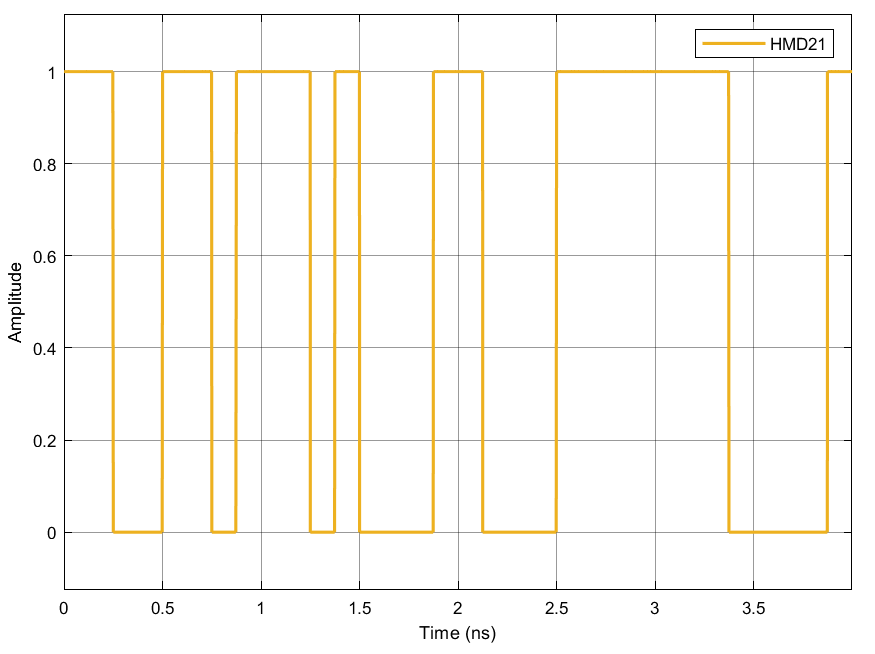
\includegraphics[width=0.5\textwidth]		
		{./sdf/m_qam_system/figures/simulations/01_noISI/HMD21.pdf}
	\caption{Signal HMD21, containing the decoded 
	bitstream.}\label{fig:ISIhmd21}
\end{figure}

	\begin{figure}[H]
		\centering
		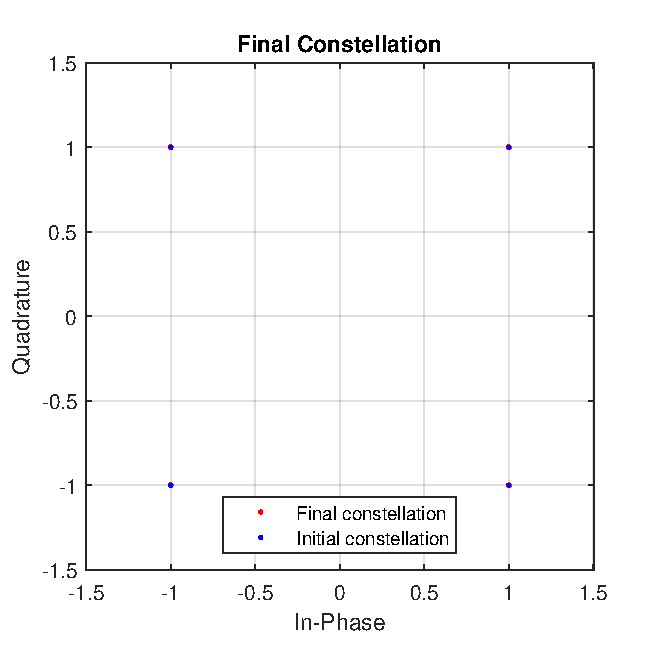
\includegraphics[width=0.7\textwidth]
		{sdf/m_qam_system/figures/simulations/01_noISI/constFinal.pdf}
	\caption{  Constellation of the encoded and decoded 
		signals. They are exactly equal due to lack of ISI and 
		noise.}\label{fig:ISIconsts}
\end{figure}

We can see that the received constellation is almost equal to the transmitted 
one, with all received 
bits having nearly no variation from their amplitude value. However, looking 
closely, we can still see a bit of the red points in 
figure~\ref{fig:ISIconsts}. This a consequence of the finite impulse response 
of the 
used filters. The ideal filters, which provide zero ISI, have infinite impulse 
response. 

\begin{figure}[H]
	\centering
	\begin{minipage}{0.3\textwidth}
		\centering
		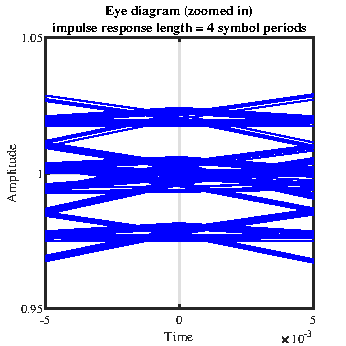
\includegraphics[width=1\textwidth]		
		{./sdf/m_qam_system/figures/simulations/01_noISI/ISI_4symbolPeriodsZoomed.pdf}
		\subcaption{}\label{fig:ISI4sp}
	\end{minipage}
	\begin{minipage}{0.3\textwidth}
		\centering
		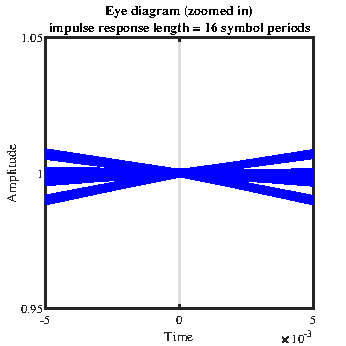
\includegraphics[width=1\textwidth]
		{sdf/m_qam_system/figures/simulations/01_noISI/ISI_16symbolPeriodsZoomed.pdf}
		\subcaption{}\label{fig:ISI16sp}
	\end{minipage}
	\begin{minipage}{0.3\textwidth}
		\centering
		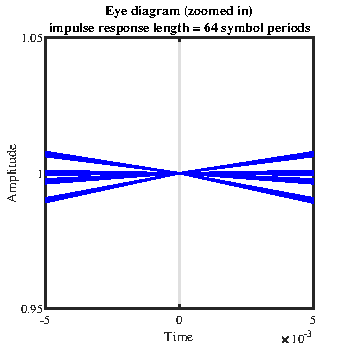
\includegraphics[width=1\textwidth]
		{sdf/m_qam_system/figures/simulations/01_noISI/ISI_64symbolPeriodsZoomed.pdf}
		\subcaption{}\label{fig:ISI64sp}
	\end{minipage}
	\caption{Zoom in on the eye diagram at sampling time. The figures used 
	filter impulse responses with lengths of (\subref{fig:ISI4sp}) 4, 
	(\subref{fig:ISI16sp})16 and 
	(\subref{fig:ISI64sp}) 64 symbol periods. As the filter impulse 
	response increases in size, the vestigial amount of ISI 
	diminishes.}\label{fig:ISIdemo}
\end{figure}

However, the practical implementation of the FIR filter implies that 
the impulse response is finite, leading to very small variations at sampling 
time. This effect can be diminished by using a larger impulse response. We have 
conducted the simulations using impulse responses with a size of 16 symbol 
periods. We can see in Figure~\ref{fig:ISI16sp} that this effect is not 
particularly significant for this situation, and thus we can consider the 
intersymbol interference to be negligible.

\subsubsection{Simulation results - Thermal 
Noise}\label{sec:simRes_thermalNoise}
After showing that the implemented shaping process does not create any 
inter-symbol interference, we will now verify the effects of electrical noise.
Electrical noise can  have several origins. For now, we will only consider 
thermal noise.

Thermal noise in the simulation will be modeled with a additive white Gaussian 
noise source, added after immediately before the sampler. According to this, 
thermal noise will not be affected by either the amplifier or matched filter, 
directly affecting the sampled signal. In addition, it is considered that the 
noise power is constant for a given temperature, which we shall consider to be 
290 K. 

The effect of this noise source is to establish a limit to the detection 
performance. Without any noise, the detected constellation could always be 
replicated perfectly, even if scaled down with the optical output power. Having 
a constant noise source makes it so that signals below a given output power 
will not be properly detected, being indistinguishable from noise.

	\begin{longtable}[h]{|l|l|l|}
	\caption{Simulation parameters\label{tab:simParams_thermal}}\\\hline
	\textbf{Parameter}            & \textbf{Value}       &\textbf{Units}\\\hline
	numberOfBitsGenerated         & $100 \times 10^3$    & \\\hline
	samplingRate                  & $64 \times 10^9$     & Hz \\\hline
	symbolRate                    & $4 \times 10^9$      & Bd \\\hline
	samplesPerSymbol              & 16                   & \\\hline
	symbolPeriod                  & $250\times 10^{-12}$ & s\\\hline
	bitPeriod                     & $125\times 10^{-12}$ & s\\\hline
	signalOutputPower\_dBm        & -6                   & dBm\\\hline
	localOscillatorPower\_dBm     & 0                    & dBm\\\hline
	localOscillatorPhase          & 0                    & rad\\\hline
	nBw                           & $18\times10^9$       & Hz\\\hline
	responsivity                  & 1                 & A/W\\\hline
	amplification                 & 0                    & \\\hline
	amplifierInputNoisePowerSpectralDensity & 0 & \\\hline
	thermalNoisePower             & 2.56248e-08          & \\\hline
	rxResistance                  & 50 & $\Omega$\\\hline
	temperatureKelvin             & 290 & K\\\hline
	outputFilter                  & RootRaisedCosine     & \\\hline
	shaperFilter                  & RootRaisedCosine     & \\\hline
	rollOffFactor\_out            & 0.9                  & \\\hline
	rollOffFactor\_shp            & 0.9                  & \\\hline
	seedType                      & RandomDevice         & \\\hline
	numberOfBitsReceived          & -1                   & \\\hline
	elFilterType                  & Defined              & \\\hline
	fiberLength\_m                & $0$                  & m \\\hline
	fiberAttenuation\_m           & 4.6052e-05           & $m^{-1}$ \\\hline
	elFilterOrder                 & 20                   & \\\hline
	opticalGain\_dB               & 0                    & dB \\\hline
	noiseFigure                   & 0                    & dB \\\hline
	bufferLength                  & 512                  & \\\hline
	bitSourceMode                 & Random               & \\\hline
	confidence                    & 0.95                 & \\\hline
\end{longtable}

The transmitted signal is similar to the one shown in 
section~\ref{sec:simRes_ISI}, so it shall not be shown here.  The starting 
constellation is also similar to the one in the previous section.
Figure~\ref{fig:sim_thermalHmd0506} shows the output of the photodiodes.

	\begin{figure}[H]
	\centering
	\begin{minipage}{0.45\textwidth}
		\centering
		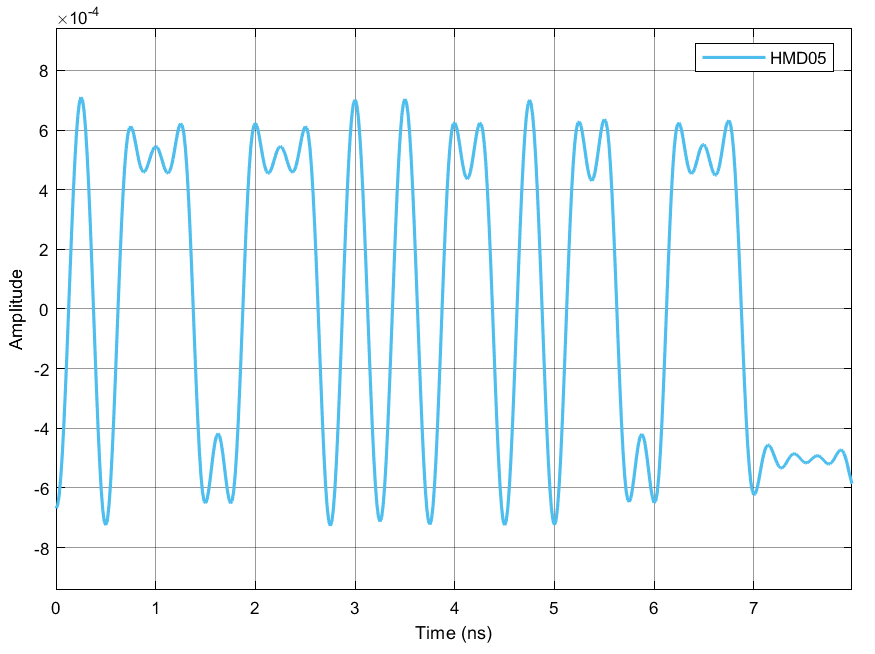
\includegraphics[width=1\textwidth]		
		{./sdf/m_qam_system/figures/simulations/02_thermal/HMD05.pdf}
		\subcaption{}\label{fig:sim_thermalHmd05}
	\end{minipage}
	\begin{minipage}{0.45\textwidth}
		\centering
		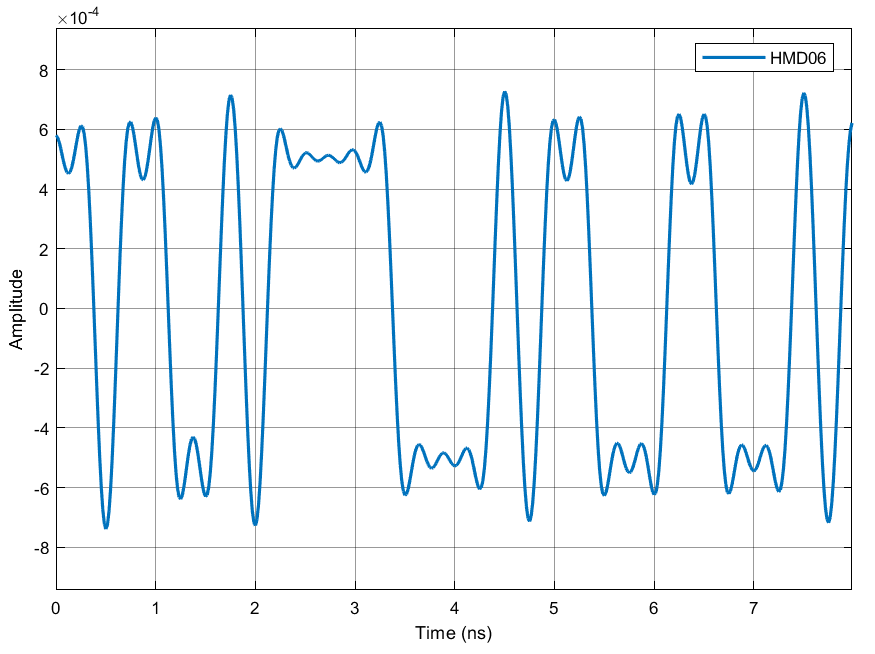
\includegraphics[width=1\textwidth]
		{sdf/m_qam_system/figures/simulations/02_thermal/HMD06.pdf}
		\subcaption{}\label{fig:sim_thermalHmd06}
	\end{minipage}
	\caption{Signals HMD05~(\subref{fig:sim_thermalHmd05}) and 
		HMD06~(\subref{fig:sim_thermalHmd06}), outputs of the 
		photodiodes.}\label{fig:sim_thermalHmd0506}
\end{figure}

In this case no signal amplification is used, so there is no amplifier gain or 
noise. This means that the electrical signal will be much smaller than in the 
previous case. This can be verified by comparing 
Figures~\ref{fig:sim_thermalHmd0910} and~\ref{fig:ISIhmd0910}.

	\begin{figure}[H]
	\centering
	\begin{minipage}{0.45\textwidth}
		\centering
		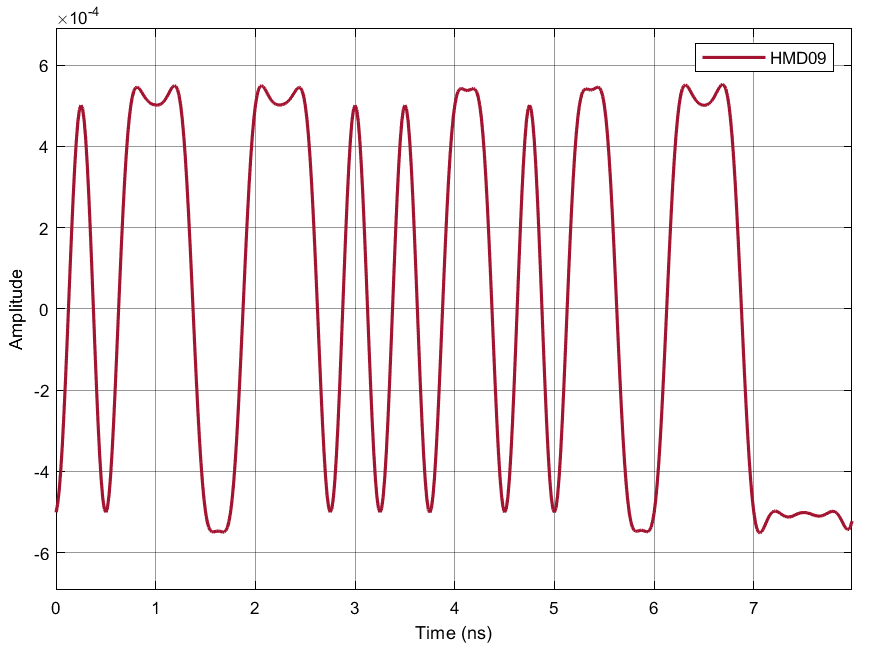
\includegraphics[width=1\textwidth]		
		{./sdf/m_qam_system/figures/simulations/02_thermal/HMD09.pdf}
		\subcaption{}\label{fig:sim_thermalHmd09}
	\end{minipage}
	\begin{minipage}{0.45\textwidth}
		\centering
		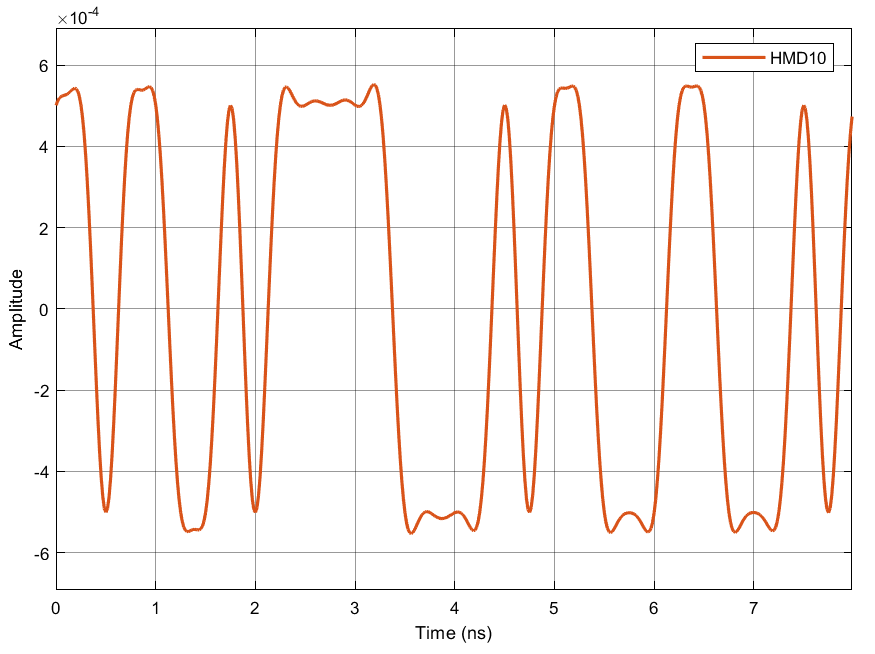
\includegraphics[width=1\textwidth]
		{sdf/m_qam_system/figures/simulations/02_thermal/HMD10.pdf}
		\subcaption{}\label{fig:sim_thermalHmd10}
	\end{minipage}
	\caption{Signals HMD09~(\subref{fig:sim_thermalHmd09}) and 
		HMD10~(\subref{fig:sim_thermalHmd10}), after the root-raised-cosine matched 
		filter. They are now following a raised-cosine 
		shape.}\label{fig:sim_thermalHmd0910}
\end{figure}

The thermal noise is then added after the matched filter. As it is only added 
at this point, it is not attenuated or filtered before the sampling process.

	\begin{figure}[H]
	\centering
	\begin{minipage}{0.45\textwidth}
		\centering
		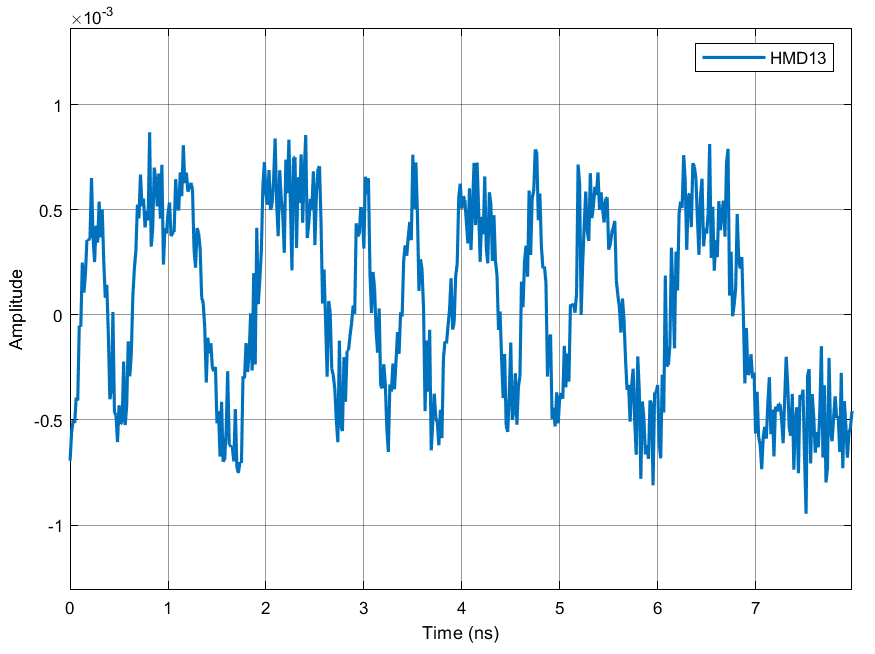
\includegraphics[width=1\textwidth]		
		{./sdf/m_qam_system/figures/simulations/02_thermal/HMD13.pdf}
		\subcaption{}\label{fig:sim_thermalHmd13}
	\end{minipage}
	\begin{minipage}{0.45\textwidth}
		\centering
		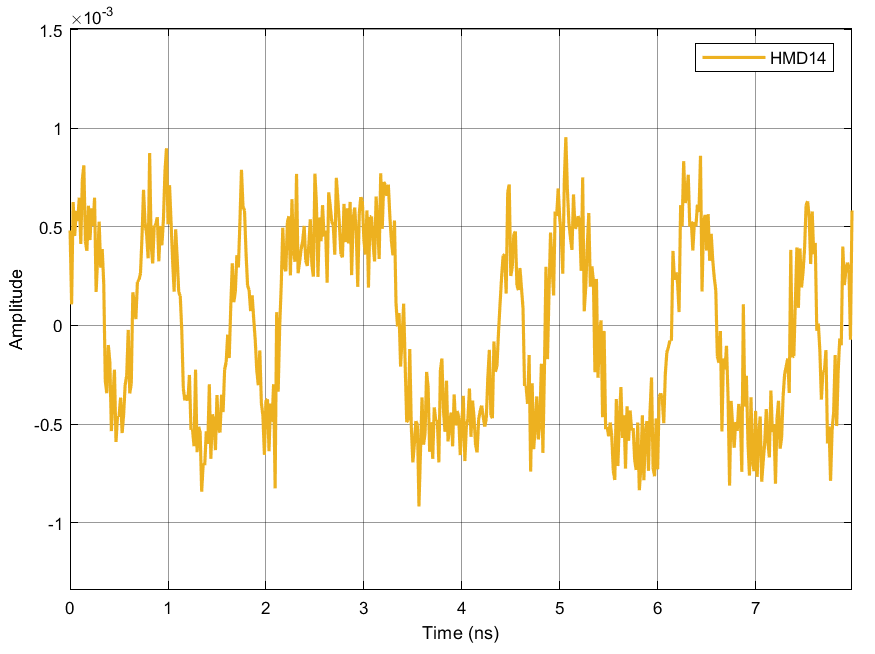
\includegraphics[width=1\textwidth]
		{sdf/m_qam_system/figures/simulations/02_thermal/HMD14.pdf}
		\subcaption{}\label{fig:sim_thermalHmd14}
	\end{minipage}
	\caption{Signals HMD13~(\subref{fig:sim_thermalHmd13}) and 
		HMD14~(\subref{fig:sim_thermalHmd14}), after adding thermal 
		noise with an RMS voltage amplitude of $1.6008 \times 10^{-4}$ 
		V.}\label{fig:sim_thermalHmd1314}
\end{figure}

	\begin{figure}[H]
	\centering
	\begin{minipage}{0.45\textwidth}
		\centering
		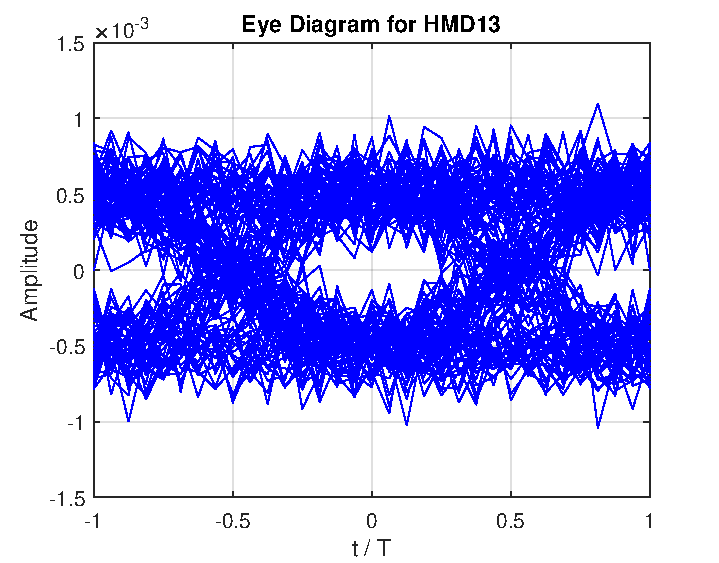
\includegraphics[width=1\textwidth]		
		{./sdf/m_qam_system/figures/simulations/02_thermal/HMD13ed.pdf}
		\subcaption{}\label{fig:sim_thermalHmd13ed}
	\end{minipage}
	\begin{minipage}{0.45\textwidth}
		\centering
		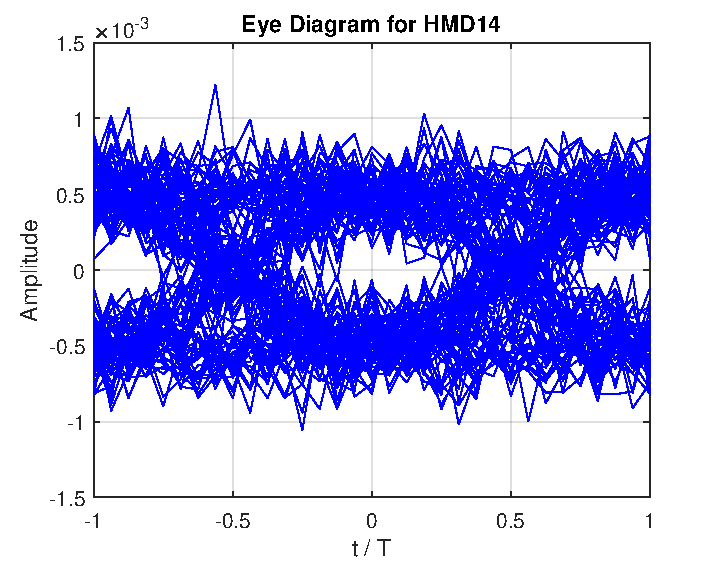
\includegraphics[width=1\textwidth]
		{sdf/m_qam_system/figures/simulations/02_thermal/HMD14ed.pdf}
		\subcaption{}\label{fig:sim_thermalHmd14ed}
	\end{minipage}
	\caption{Eye diagrams of signals HMD13~(\subref{fig:sim_thermalHmd13ed}) and 
		HMD14~(\subref{fig:sim_thermalHmd14ed}), after adding thermal 
		noise with an RMS voltage amplitude of $1.6008 \times 10^{-4}$ 
		V.}\label{fig:sim_thermalHmd1314ed}
\end{figure}

Figure~\ref{fig:thermalConsts} shows the final received constellations. Two 
things are worth noting:

\begin{itemize}
\item The amplitude of the received constellation points 
($~1\times 10^{-3}$) is much smaller than the initial constellation due to 
the lack of any amplification;
\item The received signal and constellations are strongly affected by noise. 
The thermal noise is not a particularly strong source of noise: However, as the 
signal has not been amplified, they have comparable values.
\end{itemize}


	\begin{figure}[H]
	\centering
		\begin{minipage}{0.45\textwidth}
		\centering
		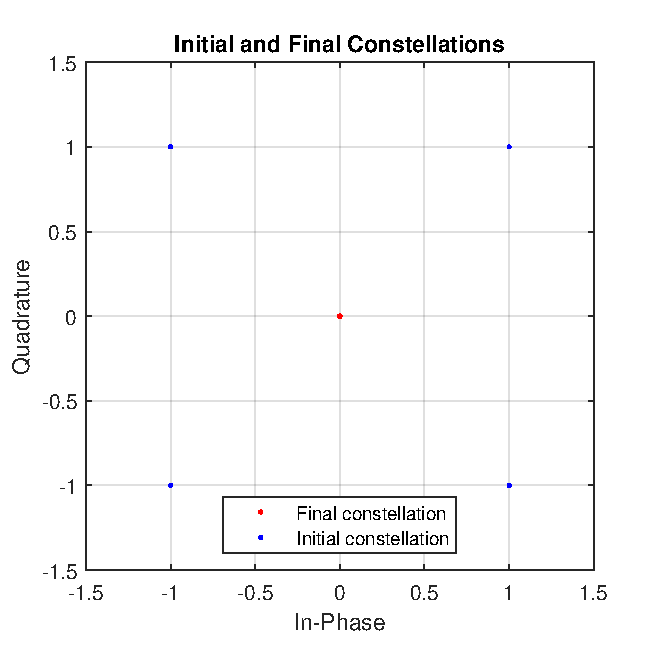
\includegraphics[width=1\textwidth]
		{sdf/m_qam_system/figures/simulations/02_thermal/constFinal_full.pdf}
		\subcaption{}\label{fig:thermalConstsFull}
	\end{minipage}
	\begin{minipage}{0.45\textwidth}
	\centering
	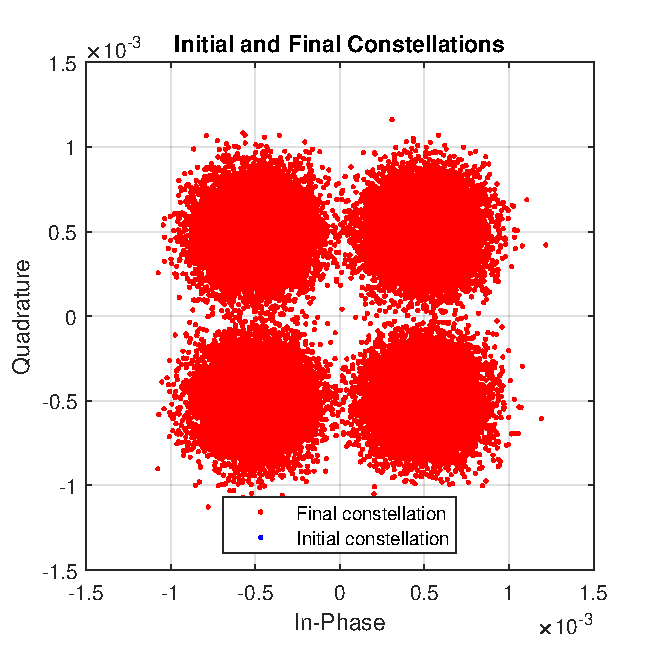
\includegraphics[width=1\textwidth]
	{sdf/m_qam_system/figures/simulations/02_thermal/constFinal.pdf}
	\subcaption{}\label{fig:thermalConstsSingle}
	\end{minipage}
	\caption{(\subref{fig:thermalConstsFull}) Comparison of transmitted and 
		received constellations. (\subref{fig:thermalConstsSingle}) Constellation 
		of 
		the decoded 
		signals.  Signal optical output power of 0 dBm and 30 km of 
		fiber length (-6 dBm at receiver input).}\label{fig:thermalConsts}
\end{figure}

The signals shown so far had an optical output power of -6 dBm. By 
attenuating using various fiber lengths, we plot a BER curve to study
receiver sensitivity. Receiver sensitivity is usually defined as the minimum 
signal optical power required to achieve a certain BER performance 
\cite{hui09}. The target BER used to measure the sensitivity may vary, and is 
usually chosen considering a desired minimum performance. For instance, in some 
cases a BER smaller than $10^{-12}$ may be desirable to ensure a very low error 
rate. In other cases, the requirement may be only $10^{-3}$ in order for the 
FEC to be effective.

In our case, there is no FEC, and the target BER value can 
be arbitrarily chosen to compare the different configurations. Therefore, we 
use choose to consider the minimum optical signal power required to reach a BER 
of $10^{-3}$. This choice was made in order to allow reaching the values 
relatively quick, with a small confidence interval. This way, generating $10^5$ 
bits we can get an average of 100 errors, which is important for the 
measurement precision. In order to achieve the same with a BER of 
$10^{-6}$ we would need to generate $10^8$ bits, likely requiring several days 
to obtain a single datapoint from the simulation.

%The sensitivity for this configuration is -4.175 dBm.

	\begin{figure}[H]
	\centering
	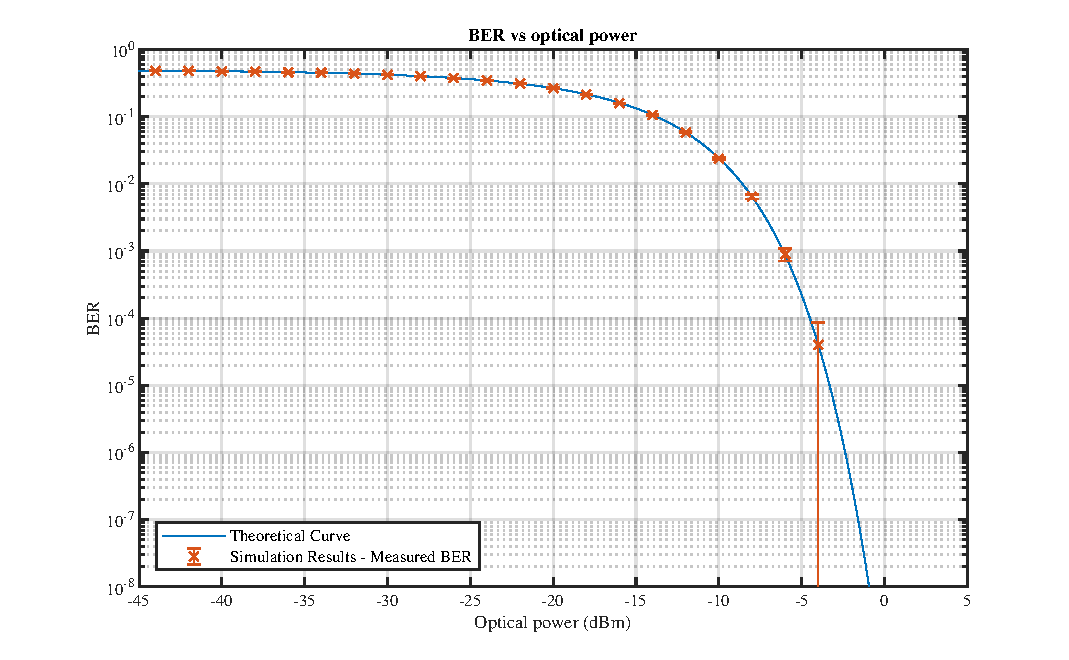
\includegraphics[width=1\textwidth]
	{sdf/m_qam_system/figures/simulations/02_thermal/berVsOpticalPower.pdf}
	\caption{BER curve of the receiver with thermal 
	noise.}\label{fig:sim_thermal_berVsOpticalPower}
\end{figure}

The theoretical curve was obtained with

\begin{equation}\label{eq:berAN}
\text{BER} = \frac{1}{2} \text{erfc} \left(\frac{A}{\sqrt{2 N}}\right) 
\end{equation}

with

\begin{align*}
A &= \eta K \sqrt{P_{LO} P_s e^{-L\alpha}} \\
N &= {4 k_B T B R}
\end{align*}

\noindent where $\eta$ is the responsivity, $P_s$ is the optical output power, 
$P_{LO}$ is the local oscillator optical output power, $L$ is the fiber length, 
$\alpha$ is the attenuation constant and K is a constant related to the matched 
filter energy. The thermal noise power $N$ is calculated as shown, where $k_B$ 
is the Boltzmann constant, T is the absolute temperature in Kelvin, B is the 
bandwidth and $R$ is the resistance.

For the sensitivity value to meaningful, in addition to the power and BER we 
should also specify the conditions in which those values were measured in the 
receiver, such as the data rate. We can therefore say the sensibility values 
presented here are obtained for a BER of $10^-3$, using a 4 GBd QPSK.

The sensitivity considering the thermal noise establishes the baseline 
sensitivity upon which to compare the rest of them. In the mentioned 
conditions, we have measured a sensibility of -6.1 dBm when using no 
amplification. We can use this value to compare with the rest of the 
simulations, in order to quantify the increased performance provided by 
improvements on the system.



\subsubsection{Simulation results - Electrical Noise}\label{sec:simRes_eNoise}

Keeping the thermal noise, we will now add a transimpedance amplifier after 
each photodiode. The amplifier has a certain bandwidth, gain and input referred 
noise. We assume that the noise gain is equal to the signal gain in this 
amplifier.

	\begin{longtable}[h]{|l|l|l|}
	\caption{Simulation parameters\label{tab:simParams_eNoise_varAmp}}\\\hline
	\textbf{Parameter}            & \textbf{Value}       &\textbf{Units}\\\hline
	numberOfBitsGenerated         & $100 \times 10^3$    & \\\hline
	samplingRate                  & $64 \times 10^9$     & Hz \\\hline
	symbolRate                    & $4 \times 10^9$      & Bd \\\hline
	samplesPerSymbol              & 16                   & \\\hline
	symbolPeriod                  & $250\times 10^{-12}$ & s\\\hline
	bitPeriod                     & $125\times 10^{-12}$ & s\\\hline
	signalOutputPower\_dBm        & -10                  & dBm\\\hline
	localOscillatorPower\_dBm     & 0                    & dBm\\\hline
	localOscillatorPhase          & 0                    & rad\\\hline
	nBw                           & $18\times10^9$       & Hz\\\hline
	responsivity                  & 1                    & A/W\\\hline
	amplification                 & 300    
	              & \\\hline
	amplifierInputNoisePowerSpectralDensity & $1.5657 \times 10^{-19}$ & \\\hline
	thermalNoisePower             & $2.56248 \times 10^{-8}$          & \\\hline
	rxResistance                  & 50 & $\Omega$\\\hline
	temperatureKelvin             & 290 & K\\\hline
	outputFilter                  & RootRaisedCosine     & \\\hline
	shaperFilter                  & RootRaisedCosine     & \\\hline
	rollOffFactor\_out            & 0.9                  & \\\hline
	rollOffFactor\_shp            & 0.9                  & \\\hline
	seedType                      & RandomDevice         & \\\hline
	numberOfBitsReceived          & -1                   & \\\hline
	elFilterType                  & Defined              & \\\hline
	fiberLength\_m                & $50 000$             & m \\\hline
	fiberAttenuation\_m           & 4.6052e-05           & $m^{-1}$ \\\hline
	elFilterOrder                 & 20                   & \\\hline
	opticalGain\_dB               & 0                    & dB \\\hline
	noiseFigure                   & 0                    & dB \\\hline
	bufferLength                  & 512                  & \\\hline
	bitSourceMode                 & Random               & \\\hline
	confidence                    & 0.95                 & \\\hline
\end{longtable}



The addition of an amplifier helps the overcome the thermal noise. 
Nevertheless, it introduces another noise source which also limits the receiver 
performance. This noise source, however, is proportional to the amplifier gain, 
so increasing the gain to very high values does not improve the sensitivity of 
the receiver.

We shall now examine the differences to the previous case. The signals up to 
the photodiodes in the receiver are similar to the previous cases. Therefore, 
we will start by showing the signals at the photodiodes. They are similar to 
the previous cases, but are a point to start.

\begin{figure}[H]
	\centering
	\begin{minipage}{0.45\textwidth}
		\centering
		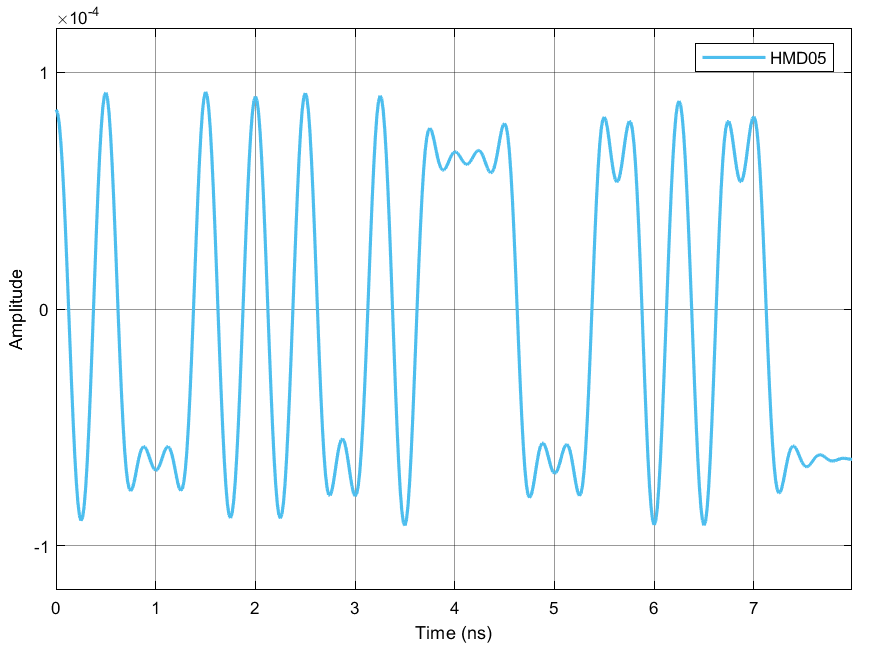
\includegraphics[width=1\textwidth]		
		{./sdf/m_qam_system/figures/simulations/03_eNoise/HMD05.pdf}
		\subcaption{}\label{fig:sim_eNoiseHmd05}
	\end{minipage}
	\begin{minipage}{0.45\textwidth}
		\centering
		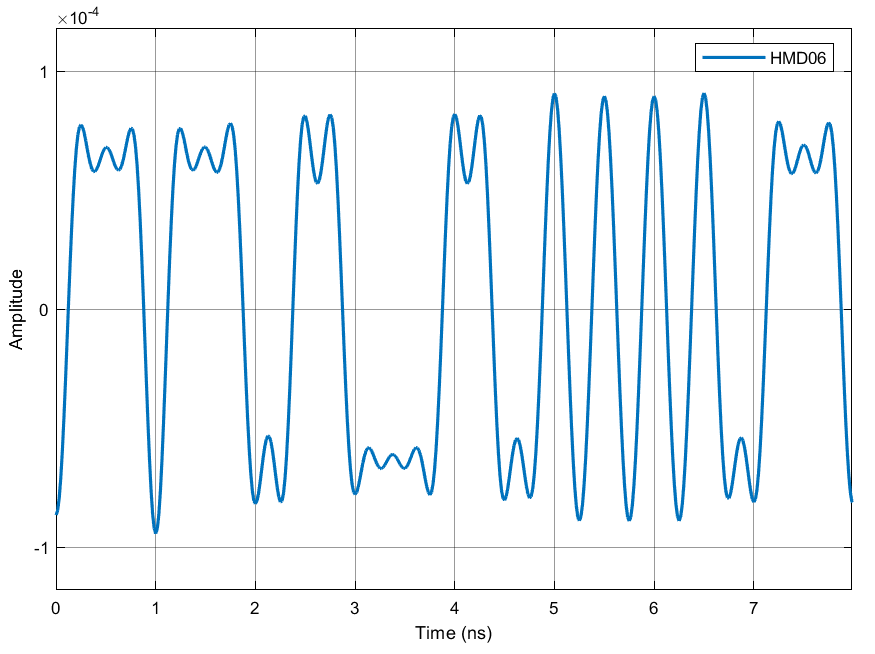
\includegraphics[width=1\textwidth]
		{sdf/m_qam_system/figures/simulations/03_eNoise/HMD06.pdf}
		\subcaption{}\label{fig:sim_eNoiseHmd06}
	\end{minipage}
	\caption{Signals HMD05~(\subref{fig:sim_eNoiseHmd05}) and 
		HMD06~(\subref{fig:sim_eNoiseHmd06}), after detection in the 
		photodiodes.}\label{fig:sim_eNoiseHmd0506}
\end{figure}


\begin{figure}[H]
	\centering
	\begin{minipage}{0.45\textwidth}
		\centering
		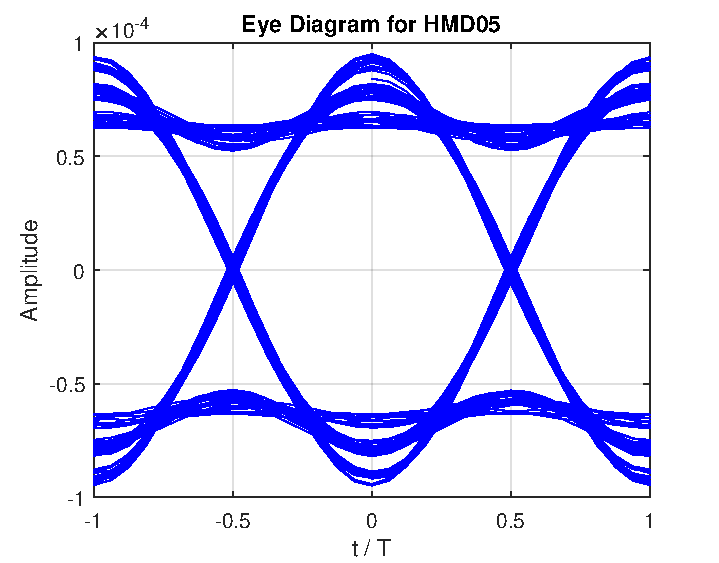
\includegraphics[width=1\textwidth]		
		{./sdf/m_qam_system/figures/simulations/03_eNoise/HMD05_ed.pdf}
		\subcaption{}\label{fig:sim_eNoiseHmd05ed}
	\end{minipage}
	\begin{minipage}{0.45\textwidth}
		\centering
		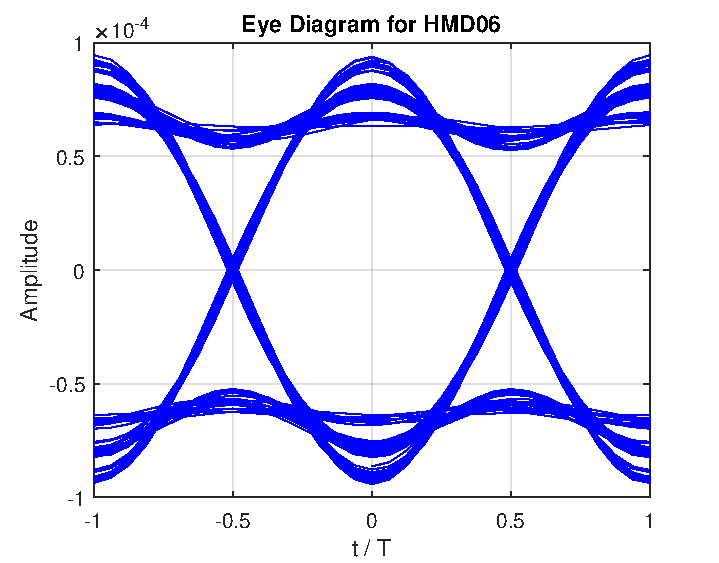
\includegraphics[width=1\textwidth]
		{sdf/m_qam_system/figures/simulations/03_eNoise/HMD06_ed.pdf}
		\subcaption{}\label{fig:sim_eNoiseHmd06ed}
	\end{minipage}
	\caption{Eye diagrams of signals HMD05~(\subref{fig:sim_eNoiseHmd05ed}) and 
		HMD06~(\subref{fig:sim_eNoiseHmd06ed}), after detection in the 
		photodiodes. Shaped with a root-raised cosine 
		filter.}\label{fig:sim_eNoiseHmd0506ed}
\end{figure}

The main difference between previous cases and this one is the existence of an 
amplifier after the photodiodes. This amplifier has three properties which 
affect the signal: a gain, an input referred noise source, and a bandwidth. The 
bandwidth is much larger than the signal bandwidth, and therefore does not have 
any appreciable effects other than limiting the noise bandwidth. The main 
effects of the amplifier, as 
shown in Figures~\ref{fig:sim_eNoiseHmd0708} and~\ref{fig:sim_eNoiseHmd0708ed}, 
are the amplification of the signal and the introduction of noise. The noise 
standard deviation increases proportionally to the amplifier gain.

\begin{figure}[H]
	\centering
	\begin{minipage}{0.45\textwidth}
		\centering
		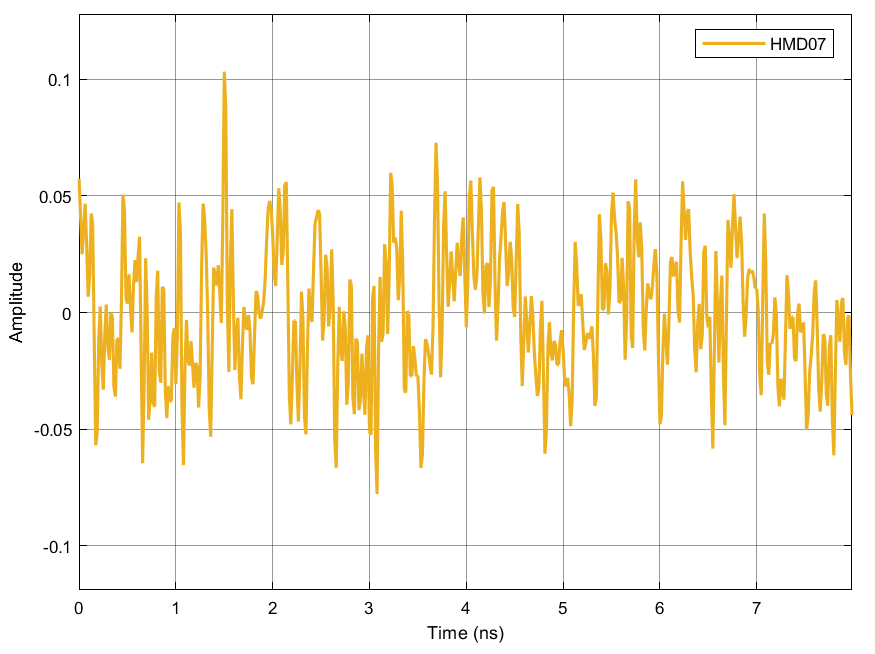
\includegraphics[width=1\textwidth]		
		{./sdf/m_qam_system/figures/simulations/03_eNoise/HMD07.pdf}
		\subcaption{}\label{fig:sim_eNoiseHmd07}
	\end{minipage}
	\begin{minipage}{0.45\textwidth}
		\centering
		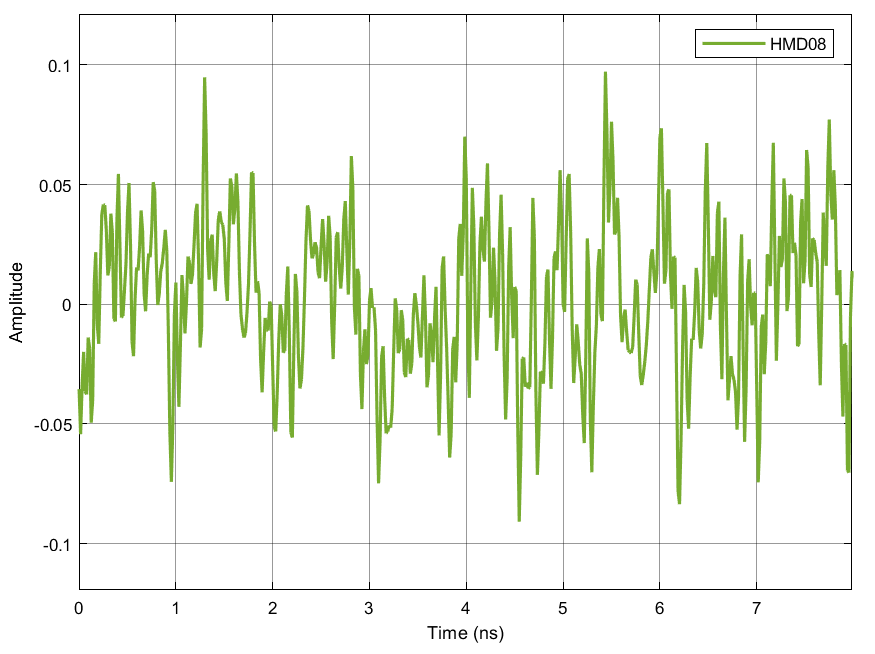
\includegraphics[width=1\textwidth]
		{sdf/m_qam_system/figures/simulations/03_eNoise/HMD08.pdf}
		\subcaption{}\label{fig:sim_eNoiseHmd08}
	\end{minipage}
	\caption{Signals HMD07~(\subref{fig:sim_eNoiseHmd07}) and 
		HMD08~(\subref{fig:sim_eNoiseHmd08}), after detection in the 
		photodiodes.}\label{fig:sim_eNoiseHmd0708}
\end{figure}


\begin{figure}[H]
	\centering
	\begin{minipage}{0.45\textwidth}
		\centering
		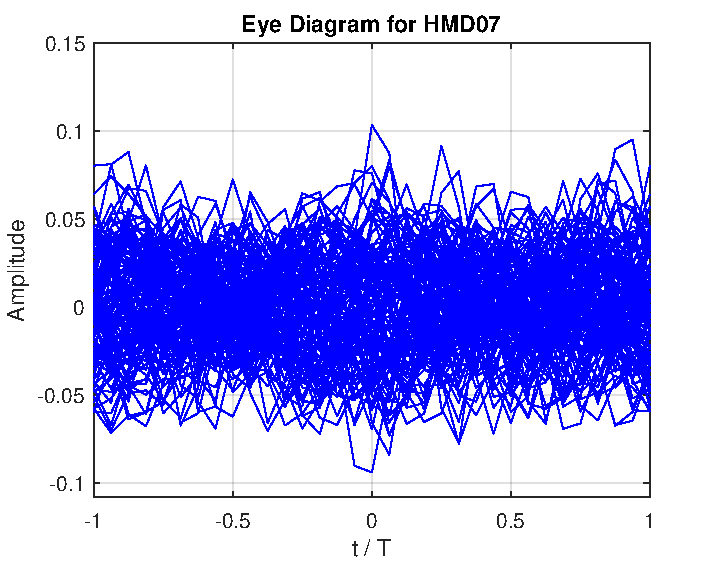
\includegraphics[width=1\textwidth]		
		{./sdf/m_qam_system/figures/simulations/03_eNoise/HMD07_ed.pdf}
		\subcaption{}\label{fig:sim_eNoiseHmd07ed}
	\end{minipage}
	\begin{minipage}{0.45\textwidth}
		\centering
		\includegraphics[width=1\textwidth]
		{sdf/m_qam_system/figures/simulations/03_eNoise/HMD08_ed.pdf}
		\subcaption{}\label{fig:sim_eNoiseHmd08ed}
	\end{minipage}
	\caption{Eye diagrams of signals HMD07~(\subref{fig:sim_eNoiseHmd07ed}) and 
		HMD08~(\subref{fig:sim_eNoiseHmd08ed}), after detection in the 
		photodiodes.}\label{fig:sim_eNoiseHmd0708ed}
\end{figure}

The new noise source is placed prior to the matched filter. As such, the noise 
is strongly attenuated when the signal goes through the matched filter. This 
can be seen particularly well by comparing the eye diagrams of 
Figures~\ref{fig:sim_eNoiseHmd0708ed} and~\ref{fig:sim_eNoiseHmd0910ed}. In the 
latter, the eye is widely open when compared to the former, and the variations 
in the signal due to noise are much smoother.

\begin{figure}[H]
	\centering
	\begin{minipage}{0.45\textwidth}
		\centering
		\includegraphics[width=1\textwidth]		
		{./sdf/m_qam_system/figures/simulations/03_eNoise/HMD09.pdf}
		\subcaption{}\label{fig:sim_eNoiseHmd09}
	\end{minipage}
	\begin{minipage}{0.45\textwidth}
		\centering
		\includegraphics[width=1\textwidth]
		{sdf/m_qam_system/figures/simulations/03_eNoise/HMD10.pdf}
		\subcaption{}\label{fig:sim_eNoiseHmd10}
	\end{minipage}
	\caption{Signals HMD09~(\subref{fig:sim_eNoiseHmd09}) and 
		HMD10~(\subref{fig:sim_eNoiseHmd10}), after detection in the 
		photodiodes.}\label{fig:sim_eNoiseHmd0910}
\end{figure}


\begin{figure}[H]
	\centering
	\begin{minipage}{0.45\textwidth}
		\centering
		\includegraphics[width=1\textwidth]		
		{./sdf/m_qam_system/figures/simulations/03_eNoise/HMD09_ed.pdf}
		\subcaption{}\label{fig:sim_eNoiseHmd09ed}
	\end{minipage}
	\begin{minipage}{0.45\textwidth}
		\centering
		\includegraphics[width=1\textwidth]
		{sdf/m_qam_system/figures/simulations/03_eNoise/HMD10_ed.pdf}
		\subcaption{}\label{fig:sim_eNoiseHmd10ed}
	\end{minipage}
	\caption{Eye diagrams of signals HMD09~(\subref{fig:sim_eNoiseHmd09ed}) and 
		HMD10~(\subref{fig:sim_eNoiseHmd10ed}), after detection in the 
		photodiodes.}\label{fig:sim_eNoiseHmd0910ed}
\end{figure}

Lastly, thermal noise is added prior to sampling. However, as can be seen in 
Figures~\ref{fig:sim_eNoiseHmd1314} and~\ref{fig:sim_eNoiseHmd1314ed}, thermal 
noise is negligible in this case, as the signal has been amplified to several 
order of magnitude above the thermal noise level.

\begin{figure}[H]
	\centering
	\begin{minipage}{0.45\textwidth}
		\centering
		\includegraphics[width=1\textwidth]		
		{./sdf/m_qam_system/figures/simulations/03_eNoise/HMD13.pdf}
		\subcaption{}\label{fig:sim_eNoiseHmd13}
	\end{minipage}
	\begin{minipage}{0.45\textwidth}
		\centering
		\includegraphics[width=1\textwidth]
		{sdf/m_qam_system/figures/simulations/03_eNoise/HMD14.pdf}
		\subcaption{}\label{fig:sim_eNoiseHmd14}
	\end{minipage}
	\caption{Signals HMD13~(\subref{fig:sim_eNoiseHmd13}) and 
		HMD14~(\subref{fig:sim_eNoiseHmd14}), after detection in the 
		photodiodes.}\label{fig:sim_eNoiseHmd1314}
\end{figure}


\begin{figure}[H]
	\centering
	\begin{minipage}{0.45\textwidth}
		\centering
		\includegraphics[width=1\textwidth]		
		{./sdf/m_qam_system/figures/simulations/03_eNoise/HMD13_ed.pdf}
		\subcaption{}\label{fig:sim_eNoiseHmd13ed}
	\end{minipage}
	\begin{minipage}{0.45\textwidth}
		\centering
		\includegraphics[width=1\textwidth]
		{sdf/m_qam_system/figures/simulations/03_eNoise/HMD14_ed.pdf}
		\subcaption{}\label{fig:sim_eNoiseHmd14ed}
	\end{minipage}
	\caption{Eye diagrams of signals HMD13~(\subref{fig:sim_eNoiseHmd13ed}) and 
		HMD14~(\subref{fig:sim_eNoiseHmd14ed}), after detection in the 
		photodiodes.}\label{fig:sim_eNoiseHmd1314ed}
\end{figure}

We then get the constellation shown in 
Figure~\ref{fig:eNoise_varAmp_constFinal}. Comparing with 
Figure~\ref{fig:thermalConsts} from the previous section, they appear to have a 
similar signal to noise ratio. While this might be true, it's worth noting that 
the constellation shown here has a much higher amplitude, equal to the 
constellation at the transmitter. In addition, it was obtained with a much 
weaker signal, -20 dBm, compared with 0 dBm in the previous example.

\begin{figure}[H]
	\centering
	\includegraphics[width=0.5\textwidth]
	{sdf/m_qam_system/figures/simulations/03_eNoise/constFinal.pdf}
	\caption{Final constellation. Signal optical output power of -20 dBm and 20 
	km of fiber length (-24 dBm at receiver 
	input).}\label{fig:eNoise_varAmp_constFinal}
\end{figure}

We can compare the results obtained here with the results from the previous 
section, where there was no amplification and only thermal noise was present. 
It is clear that the use of the amplifier leads to much better results.

	\begin{figure}[H]
	\centering
	\includegraphics[width=1\textwidth]
	{sdf/m_qam_system/figures/simulations/03_eNoise/berVsOpticalPower.pdf}
	\caption{BER curve. LO power at 0 dBm, amplifier gain set at 
	300.}\label{fig:eNoise_varAmp_berVsOpticalPower}
\end{figure}

The sensitivity at BER = $10^{-3}$ in these conditions is -22.1 dBm, which is 
quite an improvement over the unamplified scenario.

It is worth noting that the results shown here do not use the same 
amplification for all data points. Instead, the amplification in each point is 
chosen so that the signal amplitude at sampling time is equal to 1, in order to 
replicate the initial constellation.
Taking this into account, first we need to obtain the equation for the 
amplifier gain necessary to make the average of the constellation points have 
the desired value $pm A_g$ (in this case, $A_g = 1$, as it is the case on the 
initial constellation).

\begin{equation}
G_e = \frac{A_g}{\eta K \sqrt{P_s e^{-L\alpha}P_{LO}}}
\end{equation}

The curve can now be obtained with Equation~\ref{eq:berAN}, with

\begin{equation}\label{eq:berANAmped}
\begin{split}
	A &= \eta G_e K \sqrt{ P_s P_{LO} e^{-L\alpha}}\\
	N &= {4 k_B T B R} + \left(\sqrt{n_{in} \frac{1}{T_s}} G_e K\right)^2
\end{split}
\end{equation}

All variables are as previously defined. In addition, $T_s$ is the symbol 
period of the transmitted signal and $n_{in}$ is the input referred noise 
spectral density of the transimpedance amplifier.



	\begin{figure}[H]
	\centering
	\includegraphics[width=1\textwidth]
	{sdf/m_qam_system/figures/simulations/03_eNoise/berVsAmpGain.pdf}
	\caption{BER as a function of the transimpedance amplifier 
	gain, along with the curves where the individual noise sources dominate. 
	Signal output power of -25 dBm and local oscillator power of 0 dBm.
	}\label{fig:eNoise_varAmp_berVsAmpGain}
\end{figure}

	\begin{figure}[H]
	\centering
	\includegraphics[width=1\textwidth]
	{sdf/m_qam_system/figures/simulations/03_eNoise/berVsAmpGain_6dBm.pdf}
	\caption{BER as a function of the transimpedance amplifier 
		gain, along with the curves where the individual noise sources dominate. 
		Signal output power of -6 dBm and local oscillator power of 0 dBm.
	}\label{fig:eNoise_varAmp_berVsAmpGain6dBm}
\end{figure}

We can see the direct effect of the amplifier on the BER on 
Figure~\ref{fig:eNoise_varAmp_berVsAmpGain}.
The yellow curve is the expected behavior if thermal noise was the only noise 
source. It 
better demonstrates the system behavior at low gains, 
reflecting the case where the thermal noise 
overwhelms the amplifier-generated noise. As 
the gain increases, the thermal noise component becomes less significant when 
compared to the signal and to the amplifier noise. When the gain is high enough 
($10^2$ in the plot), thermal noise is negligible when compared to the 
amplifier output, and system follows the purple line. This line shows the 
expected behavior if the only noise present was due to the amplifier. At this 
point, the 
performance limiting factor is the relation between the current 
generated at the photodiodes and the input referred noise of the amplifiers. 
This ratio is constant and independent from the gain.

	\begin{figure}[H]
	\centering
	\includegraphics[width=1\textwidth]
	{sdf/m_qam_system/figures/simulations/03_eNoise/berVsOpticalPowerVar.pdf}
	\caption{Comparison of BER curves with different gains. Local oscillator 
	power of 0 dBm. We can see that when G=1, the curve is similar to the case 
	without amplifier shown in 
	Figure~\ref{fig:sim_thermal_berVsOpticalPower}}\label{fig:eNoise_varAmp_berCurveAmpGainVar}
\end{figure}

\begin{figure}[h]
	\centering
	\begin{minipage}{0.33\textwidth}
		\centering
		\includegraphics[width=1\textwidth]{sdf/m_qam_system/figures/simulations/03_eNoise/constFinal_G5_20km.pdf}
		\subcaption{$G = 5$}
	\end{minipage}
	\begin{minipage}{0.33\textwidth}
		\centering
		\includegraphics[width=1\textwidth]{sdf/m_qam_system/figures/simulations/03_eNoise/constFinal_G10_20km.pdf}
		\subcaption{$G = 10$}
	\end{minipage}
	\begin{minipage}{0.33\textwidth}
		\centering
		\includegraphics[width=1\textwidth]{sdf/m_qam_system/figures/simulations/03_eNoise/constFinal_G100_20km.pdf}
		\subcaption{$G = 100$}
	\end{minipage}
	\begin{minipage}{0.33\textwidth}
		\centering
		\includegraphics[width=1\textwidth]{sdf/m_qam_system/figures/simulations/03_eNoise/constFinal_G1000_20km.pdf}
		\subcaption{$G = 1000$}
	\end{minipage}
	\caption{Final constellations for various local oscillator optical 
		powers. Signal optical power at is -15 
		dBm, with 20 km of fiber length (-19 dBm at receiver 
		input). It is easy to see that there does not appear to be a significant 
		improvement between the constellations with the gains of 100 and 
		1000.}\label{fig:sim_eNoise_consts}
\end{figure}

\clearpage


\subsubsection{Simulation results - Increased LO}\label{sec:simRes_incLO}

As mentioned in the previous section, one way to further increase performance 
is to improve the relation between the current generated at the photodiodes and 
the input referred noise of the amplifiers. This can be done by using a higher 
optical power on the Local Oscillator. Thus, the current generated at the 
current generated at the photodiodes will be increased.

	\begin{longtable}[h]{|l|l|l|}
	\caption{Simulation parameters\label{tab:simParams_incLO}}\\\hline
	\textbf{Parameter}            & \textbf{Value}       &\textbf{Units}\\\hline
	numberOfBitsGenerated         & $100 \times 10^3$    & \\\hline
	samplingRate                  & $64 \times 10^9$     & Hz \\\hline
	symbolRate                    & $4 \times 10^9$      & Bd \\\hline
	samplesPerSymbol              & 16                   & \\\hline
	symbolPeriod                  & $250\times 10^{-12}$ & s\\\hline
	bitPeriod                     & $125\times 10^{-12}$ & s\\\hline
	signalOutputPower\_dBm        & -20                  & dBm\\\hline
	localOscillatorPower\_dBm     & 5                    & dBm\\\hline
	localOscillatorPhase          & 0                    & rad\\\hline
	nBw                           & $18\times10^9$       & Hz\\\hline
	responsivity                  & 1                    & A/W\\\hline
	amplification                 & 300                  & \\\hline
	amplifierInputNoisePowerSpectralDensity & $1.5657 \times 10^{-19}$ & \\\hline
	thermalNoisePower             & $2.56248 \times 10^{-8}$          & \\\hline
	rxResistance                  & 50 & $\Omega$\\\hline
	temperatureKelvin             & 290 & K\\\hline
	outputFilter                  & RootRaisedCosine     & \\\hline
	shaperFilter                  & RootRaisedCosine     & \\\hline
	rollOffFactor\_out            & 0.9                  & \\\hline
	rollOffFactor\_shp            & 0.9                  & \\\hline
	seedType                      & RandomDevice         & \\\hline
	numberOfBitsReceived          & -1                   & \\\hline
	elFilterType                  & Defined              & \\\hline
	fiberLength\_m                & $20 000$             & m \\\hline
	fiberAttenuation\_m           & 4.6052e-05           & $m^{-1}$ \\\hline
	elFilterOrder                 & 20                   & \\\hline
	opticalGain\_dB               & 0                    & dB \\\hline
	noiseFigure                   & 0                    & dB \\\hline
	bufferLength                  & 512                  & \\\hline
	bitSourceMode                 & Random               & \\\hline
	confidence                    & 0.95                 & \\\hline
\end{longtable}

The increased current at the photodiodes' output means that the same amplitude 
can be reached with a lower amplifier gain. A lower gain, by itself, implies 
that the input referred noise of the amplifier will stay at a lower value, 
thereby increasing the sensitivity of the system.
In this example, the signals will not be shown here, as the only difference is 
that the amplitude of the signal after the photodiodes is higher.

\begin{figure}[H]
	\centering
	\includegraphics[width=0.5\textwidth]
	{sdf/m_qam_system/figures/simulations/04_incLO/constFinal.pdf}
	\caption{Final constellation (normalized). Signal optical output power of -20 
	dBm and 20 
		km of fiber length (-24 dBm at receiver 
		input). Local oscillator at 5 dBm.}\label{fig:incLO_constFinal}
\end{figure}

In Figure~\ref{fig:incLO_constFinal} we can see the final constellation 
obtained when choosing an output optical power of -20 dBm and setting the fiber 
length to 20 km. In conditions similar to 
Figure~\ref{fig:eNoise_varAmp_constFinal} it shows a much better constellation. 
This is all due to the higher local oscillator value.



	\begin{figure}[H]
	\centering
	\includegraphics[width=1\textwidth]
	{sdf/m_qam_system/figures/simulations/04_incLO/berComp.pdf}
	\caption{Comparison of BER curves: considering thermal noise only, using an 
	electrical amplifier, and using a higher value of local 
	oscillator together with the amplifier. Amplifier gain was set at 
	300.}\label{fig:sim_incLO_ber12dBm}
\end{figure}

The sensitivity of the new curve, at BER $10^{-3}$,with local oscillator power 
of 5 dBm, is -27.1 dBm, 5 dB lower than the curve with the LO at 0 dBm.

The theoretical curve in Figure~\ref{fig:sim_incLO_ber12dBm} was obtained 
according to the same equation as the second curve in the previous section. 
Notice that the new curve is approximately 5 dB to the left of curve with the 
amplifier and the LO at 0 dBm. This is because in the 
equations~\ref{eq:berAN} and~\ref{eq:berANAmped}, the power of the local 
oscillator is as important as the optical signal power, and the amplitude at 
sampling time grows at the same rate with both quantities.

	\begin{figure}[h]
	\centering
	\includegraphics[width=1\textwidth]
	{sdf/m_qam_system/figures/simulations/04_incLO/berCurveVarLO.pdf}
	\caption{Variation of BER with the LO power. Signal optical power at receiver 
	input is -25 dBm.}\label{fig:sim_incLO_varLO}
\end{figure}

\begin{figure}[h]
	\centering
	\begin{minipage}{0.33\textwidth}
		\centering
		\includegraphics[width=1\textwidth]{sdf/m_qam_system/figures/simulations/04_incLO/constNorm_lo0dBm.pdf}
		\subcaption{$P_{lo} = 0$ dBm}
	\end{minipage}
	\begin{minipage}{0.33\textwidth}
		\centering
		\includegraphics[width=1\textwidth]{sdf/m_qam_system/figures/simulations/04_incLO/constNorm_lo3dBm.pdf}
		\subcaption{$P_{lo} = 3$ dBm}
	\end{minipage}
	\begin{minipage}{0.33\textwidth}
		\centering
		\includegraphics[width=1\textwidth]{sdf/m_qam_system/figures/simulations/04_incLO/constNorm_lo6dBm.pdf}
		\subcaption{$P_{lo} = 6$ dBm}
	\end{minipage}
	\begin{minipage}{0.33\textwidth}
		\centering
		\includegraphics[width=1\textwidth]{sdf/m_qam_system/figures/simulations/04_incLO/constNorm_lo20dBm.pdf}
		\subcaption{$P_{lo} = 20$ dBm}
	\end{minipage}
	\caption{Final constellations for various local oscillator optical 
		powers. Signal optical power at receiver input is -25 
		dBm.}\label{fig:sim_loVarConsts}
\end{figure}

This might lead us to believe that by increasing the LO, the performance can be 
improved as much as required. However, that would only be the case if the Local 
	Oscillator was independent from any noise source. That is not the case, as we 
shall see in the next section.

\clearpage

\subsubsection{Simulation results - Quantum 
Noise}\label{sec:simRes_quantumNoise}

We will now consider the more realistic case when there is quantum noise 
associated with the local oscillator. We can consider quantum noise to be 
similar to shot noise.

In this simulation, we will add noise at the photodiodes, where the noise 
current variance will be proportional to total generated photocurrent. 
Normally, shot noise follows a Poisson distribution. However, for the purpose 
of this section, we shall consider that the number of photons is high enough so 
that it can be considered to follow a normal distribution.

\begin{equation}
\sigma_{\text{shot}}^2 = 2 q I B = 2 \eta P_\text{opt} B
\end{equation}

As the local oscillator will be much higher than the signal, we can consider 
that the total optical power generating current is equal to the local 
oscillator power. Due to the optical hybrid, each photodiode receives $1/4$ of 
the local oscillator optical power.

Keeping in mind that the noise and signal will be affected by the same gains, 
the factor which control performance are the signal and noise ratio at the 
photodiodes output, and the matched filter. The other blocks of the receiver 
will have no practical effects, as the LO amplification will render the other 
noise sources negligible, and the matched filter ultimately limits the noise 
bandwidth.

We then have that the signal current amplitude at the photodiode's output is 
given by:

\begin{equation}
	A = \eta \sqrt{ P_{LO} P_s }
\end{equation}


On the other hand, the shot noise variance $N_\text{shot i}$ in each photodiode 
will be given by

\begin{equation}
	N_{\text{shot i}} = 2 \eta h f \frac{P_{LO}}{4} B
\end{equation}

\noindent with $2 B = 1/\tau$, where $\tau$ is the sampling period.

Considering the shot noise to be approximated as a gaussian random 
variable, the noise at output of each pair of photodiodes can be obtained by 
the sum of their variances:

\begin{equation}
	\begin{split}
		N_{\text{shot}} &= N_{\text{shot 1}} + N_{\text{shot 2}} \\
										&\approxeq 2 N_{\text{shot i}} =\\
										&= 4 \eta h f \frac{P_{LO}}{4} B
	\end{split}
\end{equation}

We can now calculate $A$ and $N$ after the matched filter output:

\begin{equation}
	\begin{split}
		A &= \eta G_e K \sqrt{ P_s P_{LO} e^{-L\alpha}}\\
		N &= {4 k_B T B R} + \left(\sqrt{n_{in} \frac{1}{T_s}} G_e K\right)^2 +
		 \left(\sqrt{\frac{N_{\text{shot}}}{B} \frac{1}{T_s}} G_e K\right)^2
	\end{split}
\end{equation}

	\begin{figure}[h]
	\centering
	\includegraphics[width=1\textwidth]
	{sdf/m_qam_system/figures/simulations/05_loShot/berCurve_loShotVar.pdf}
	\caption{Variation of BER with the LO power, with shot noise. Signal optical 
	power at receiver 
		input is -56 dBm.}\label{fig:sim_loShot_varLO}
\end{figure}

In addition, we can compare these results with the quantum limit. The quantum 
limit establishes the absolute minimum sensitivity of the receiver, and varies 
according to the modulation scheme and type of detector. In the case of QPSK 
with homodyne detection this limit is given by~\cite{senior09, agrawal12}:

\begin{equation}\label{eq:quantumLimit_homodyne}
\text{BER} = \frac{1}{2} \text{erfc}\left( \sqrt{2 \eta_q N_p}\right)
\end{equation}

\noindent where $eta_q$ is the quantum efficiency of the receiver, and $N_p$ is 
the number of photons per bit. We can convert the average number of photons per 
bit to dBm or vice versa:

\begin{align}
	P_{\text{dBm}} = 10 \log_{10}\left(\frac{h f}{T_b} N_p \times 10^3\right) \\
	N_p = \frac{10^{(P_{\text{dBm}}/10)} T_b \times 10^{-3}}{hf}
\end{align}

It is worth remembering that we are neglecting most effects which arise due to 
working with a small number of photons, and just assuming that the system 
behaves similarly as for larger numbers of photons.

	\begin{figure}[h]
	\centering
	\includegraphics[width=1\textwidth]
	{sdf/m_qam_system/figures/simulations/05_loShot/berCurve_loShot2.pdf}
	\caption{BER variation with the optical power. $P_{lo} = 50$ dBm 
	.}\label{fig:sim_loShot_quantumLimit}
\end{figure}

We can see that in this case the sensitivity at a BER $10^{-3}$ is -56 dBm, 
which is at the quantum limit. This corresponds to an average of 2.4 photons 
per bit.

%
%The main 
%difference is on the signal after the matched filter, which is affected by 
%noise. Signals HMD09 and HMD10 then become as shown in 
%Figures~\ref{fig:sim_thermalHmd0910} and~\ref{fig:sim_thermalHmd0910ed}.
%
%	\begin{figure}[H]
%	\centering
%	\begin{minipage}{0.45\textwidth}
%		\centering
%		\includegraphics[width=1\textwidth]		
%		{./sdf/m_qam_system/figures/simulations/02_thermal/HMD09.pdf}
%		\subcaption{}\label{fig:sim_thermalHmd09}
%	\end{minipage}
%	\begin{minipage}{0.45\textwidth}
%		\centering
%		\includegraphics[width=1\textwidth]
%		{sdf/m_qam_system/figures/simulations/02_thermal/HMD10.pdf}
%		\subcaption{}\label{fig:sim_thermalHmd10}
%	\end{minipage}
%	\caption{Eye diagrams for HMD09~(\subref{fig:ISIhmd09ed}) and 
%		HMD10~(\subref{fig:ISIhmd10ed}), after the root-raised-cosine matched 
%		filter. They are now following a raised-cosine 
%		shape.}\label{fig:sim_thermalHmd0910}
%\end{figure}
%
%	\begin{figure}[H]
%	\centering
%	\begin{minipage}{0.45\textwidth}
%		\centering
%		\includegraphics[width=1\textwidth]		
%		{./sdf/m_qam_system/figures/simulations/02_thermal/HMD09_ed.pdf}
%		\subcaption{}\label{fig:sim_thermalHmd09ed}
%	\end{minipage}
%	\begin{minipage}{0.45\textwidth}
%		\centering
%		\includegraphics[width=1\textwidth]
%		{sdf/m_qam_system/figures/simulations/02_thermal/HMD10_ed.pdf}
%		\subcaption{}\label{fig:sim_thermalHmd10ed}
%	\end{minipage}
%	\caption{Eye diagrams for HMD09~(\subref{fig:ISIhmd09ed}) and 
%		HMD10~(\subref{fig:ISIhmd10ed}), after the root-raised-cosine matched 
%		filter. They are now following a raised-cosine 
%		shape.}\label{fig:sim_thermalHmd0910ed}
%\end{figure}


%\subsubsection{Simulation results - Electrical Noise}\label{sec:simRes_eNoise}
%
%After showing that the implemented shaping process does not create any 
%inter-symbol interference, we will now verify the effects of electrical noise.
%This noise currently has two components:
%
%\begin{itemize}
%	\item The transimpedance amplifier block generates electrical noise dependent 
%	on the gain. In real world datasheets, this noise is quantified as, for 
%	instance, an input referred noise current. This current is then amplified, 
%	depending on the gain of the amplifier. In model we use, the gain is equal 
%	for the signal and for the noise.
%	\item White noise modeling thermal voltage noise is also generated after the 
%	amplifier, and added to the signal.
%\end{itemize}
%
%We shall see the effects of these noise sources, and how they affect 
%the simulated system's performance.
%
%	\begin{longtable}[h]{|l|l|l|}
%	\caption{Simulation parameters\label{tab:fiberThermalParams}}\\\hline
%	\textbf{Parameter}            & \textbf{Value}       &\textbf{Units}\\\hline
%	numberOfBitsGenerated         & $100 \times 10^3$    & \\\hline
%	samplingRate                  & $64 \times 10^9$     & Hz \\\hline
%	symbolRate                    & $4 \times 10^9$      & Bd \\\hline
%	samplesPerSymbol              & 16                   & \\\hline
%	symbolPeriod                  & $250\times 10^{-12}$ & s\\\hline
%	bitPeriod                     & $125\times 10^{-12}$ & s\\\hline
%	signalOutputPower\_dBm        & -10                  & dBm\\\hline
%	localOscillatorPower\_dBm     & 0                    & dBm\\\hline
%	localOscillatorPhase          & 0                    & rad\\\hline
%	nBw                           & $18\times10^9$       & Hz\\\hline
%	responsivity                  & 0.05                 & A/W\\\hline
%	amplification                 & 39529.1              & \\\hline
%	amplifierInputNoisePowerSpectralDensity & 3.1314e-23 & \\\hline
%	thermalNoisePowerSpectralDensity& 1.6015520e-18      & \\\hline
%	rxResistance                  & 50 & $\omega$\\\hline
%	temperatureKelvin             & 290 & K\\\hline
%	outputFilter                  & RootRaisedCosine     & \\\hline
%	shaperFilter                  & RootRaisedCosine     & \\\hline
%	rollOffFactor\_out            & 0.9                  & \\\hline
%	rollOffFactor\_shp            & 0.9                  & \\\hline
%	seedType                      & RandomDevice         & \\\hline
%	numberOfBitsReceived          & -1                   & \\\hline
%	elFilterType                  & Defined              & \\\hline
%	fiberLength\_m                & $100 \times 10^3$    & m \\\hline
%	fiberAttenuation\_m           & 4.6052e-05           & $m^{-1}$ \\\hline
%	elFilterOrder                 & 20                   & \\\hline
%	opticalGain\_dB               & 0                    & dB \\\hline
%	noiseFigure                   & 0                    & dB \\\hline
%	preFilterNoiseSpectralDensity & $1 \times 10^-{17}$  & W/Hz\\\hline
%	elNoiseSpectralDensity        & 0                    & W/Hz\\\hline
%	bufferLength                  & 512                  & \\\hline
%	bitSourceMode                 & Random               & \\\hline
%	midReportSize                 & 0                    & \\\hline
%	confidence                    & 0.95                 & \\\hline
%	samplesToSkip                 & 256                  & \\\hline
%\end{longtable}
%
%
%	\begin{figure}[H]
%	\centering
%	\includegraphics[width=0.7\textwidth]
%	{sdf/m_qam_system/figures/simulations/02_eNoise/constFinal.pdf}
%	\caption{Constellation of the encoded and decoded 
%		signals. They coincide, but the received constellation is affected by some 
%		noise.}\label{fig:eNoiseconsts}
%\end{figure}
%
%\subsubsection{Simulation results - Optical Fiber with Electrical 
%	Noise}\label{sec:simRes_eNoiseAtt}
%	
%	Building upon the former example, we shall now increase the 
%	fiber length, while maintaining the electrical amplifier gain and noise 
%	spectral densities. We shall see that keeping these properties constant 
%	establishes a given relation between the optical fiber length and the bit 
%	error rate.
%		
%	Table~\ref{tab:fiberThermalParams} shows the parameters used to obtain the 
%	signals in this section.
%	
%	\begin{longtable}[h]{|l|l|l|}
%		\caption{Simulation parameters\label{tab:fiberThermalParams}}\\\hline
%		\textbf{Parameter}            & \textbf{Value}       &\textbf{Units}\\\hline
%		numberOfBitsGenerated         & $100 \times 10^3$    & \\\hline
%		samplingRate                  & $64 \times 10^9$     & Hz \\\hline
%		symbolRate                    & $4 \times 10^9$      & Bd \\\hline
%		samplesPerSymbol              & 16                   & \\\hline
%		symbolPeriod                  & $250\times 10^{-12}$ & s\\\hline
%		bitPeriod                     & $125\times 10^{-12}$ & s\\\hline
%		signalOutputPower\_dBm        & -10                  & dBm\\\hline
%		localOscillatorPower\_dBm     & 0                    & dBm\\\hline
%		localOscillatorPhase          & 0                    & rad\\\hline
%		nBw                           & $18\times10^9$       & Hz\\\hline
%		amplification                 & 40                   & \\\hline
%		responsivity                  & 0.07                 & A/W\\\hline
%		outputFilter                  & RootRaisedCosine     & \\\hline
%		shaperFilter                  & RootRaisedCosine     & \\\hline
%		rollOffFactor\_out            & 0.9                  & \\\hline
%		rollOffFactor\_shp            & 0.9                  & \\\hline
%		seedType                      & RandomDevice         & \\\hline
%		numberOfBitsReceived          & -1                   & \\\hline
%		elFilterType                  & Defined              & \\\hline
%		fiberLength\_m                & $100 \times 10^3$    & m \\\hline
%		fiberAttenuation\_m           & 4.6052e-05           & $m^{-1}$ \\\hline
%		elFilterOrder                 & 20                   & \\\hline
%		opticalGain\_dB               & 0                    & dB \\\hline
%		noiseFigure                   & 0                    & dB \\\hline
%		preFilterNoiseSpectralDensity & $1 \times 10^-{17}$  & W/Hz\\\hline
%		elNoiseSpectralDensity        & 0                    & W/Hz\\\hline
%		bufferLength                  & 512                  & \\\hline
%		bitSourceMode                 & Random               & \\\hline
%		midReportSize                 & 0                    & \\\hline
%		confidence                    & 0.95                 & \\\hline
%		samplesToSkip                 & 266                  & \\\hline
%	\end{longtable}
%	
%	The optical signals are similar to the ones shown in the previous section, so 
%	we shall skip them. We will start by looking at the signals HMD07 and HMD08, 
%	the amplified version of the signals detected at the photodiodes.
%	
%	\begin{figure}[H]
%		\centering
%		\begin{minipage}{0.45\textwidth}
%			\centering
%			\includegraphics[width=1\textwidth]		
%			{./sdf/m_qam_system/figures/simulations/04_wFiberThermal/HMD07.pdf}
%			\subcaption{}\label{fig:fiberThmd07}
%		\end{minipage}
%		\begin{minipage}{0.45\textwidth}
%			\centering
%			\includegraphics[width=1\textwidth]
%			{sdf/m_qam_system/figures/simulations/04_wFiberThermal/HMD08.pdf}
%			\subcaption{}\label{fig:fiberThmd08}
%		\end{minipage}
%		\caption{Signals HMD07~(\subref{fig:fiberThmd07}) and 
%			HMD08~(\subref{fig:fiberThmd08}), 
%			containing the amplified versions of the signals detected at the 
%			\textit{photodiode} blocks}\label{fig:fiberThmd0708}
%	\end{figure}
%	
%	So far the signals look very similar the previous ones. However, this time we 
%	add Gaussian white noise to model thermal noise at the receiver.
%	
%	\begin{figure}[H]
%		\centering
%		\begin{minipage}{0.45\textwidth}
%			\centering
%			\includegraphics[width=1\textwidth]		
%			{./sdf/m_qam_system/figures/simulations/04_wFiberThermal/HMD11.pdf}
%			\subcaption{}\label{fig:fiberThmd11}
%		\end{minipage}
%		\begin{minipage}{0.45\textwidth}
%			\centering
%			\includegraphics[width=1\textwidth]
%			{sdf/m_qam_system/figures/simulations/04_wFiberThermal/HMD12.pdf}
%			\subcaption{}\label{fig:fiberThmd12}
%		\end{minipage}
%		\caption{Signals HMD1~(\subref{fig:fiberThmd11}) and 
%			HMD12~(\subref{fig:fiberThmd12}), 
%			amplified signals after white adding noise.}\label{fig:fiberThmd1112}
%	\end{figure}
%	
%	The amount of noise is limited by the bandwidth of the electrical filter.
%	
%	\begin{figure}[H]
%		\centering
%		\begin{minipage}{0.45\textwidth}
%			\centering
%			\includegraphics[width=1\textwidth]		
%			{./sdf/m_qam_system/figures/simulations/04_wFiberThermal/HMD13.pdf}
%			\subcaption{}\label{fig:fiberThmd13}
%		\end{minipage}
%		\begin{minipage}{0.45\textwidth}
%			\centering
%			\includegraphics[width=1\textwidth]
%			{sdf/m_qam_system/figures/simulations/04_wFiberThermal/HMD14.pdf}
%			\subcaption{}\label{fig:fiberThmd14}
%		\end{minipage}
%		\caption{Signals HMD13~(\subref{fig:fiberThmd13}) and 
%			HMD14~(\subref{fig:fiberThmd14}), 
%			signals after the electrical filter.}\label{fig:fiberThmd1314}
%	\end{figure}
%	
%	In addition, the matched filter improves the SNR before sampling. However, in 
%	this case, the noise power is too high when compared with the signal.
%	
%	\begin{figure}[H]
%		\centering
%		\begin{minipage}{0.45\textwidth}
%			\centering
%			\includegraphics[width=1\textwidth]		
%			{./sdf/m_qam_system/figures/simulations/04_wFiberThermal/HMD23.pdf}
%			\subcaption{}\label{fig:fiberThmd23}
%		\end{minipage}
%		\begin{minipage}{0.45\textwidth}
%			\centering
%			\includegraphics[width=1\textwidth]
%			{sdf/m_qam_system/figures/simulations/04_wFiberThermal/HMD24.pdf}
%			\subcaption{}\label{fig:fiberThmd24}
%		\end{minipage}
%		\caption{Signals HMD23~(\subref{fig:fiberThmd23}) and 
%			HMD24~(\subref{fig:fiberThmd24}), 
%			signals after the electrical filter.}\label{fig:fiberThmd2324}
%	\end{figure}
%	
%	Looking back at the previous section, the expected amplitude at the 
%	constellation would be close to $2 \times 
%	10^{-3}$. However, looking at Figures~\ref{fig:fiberThmd2324} 
%	and~\ref{fig:fiberTconsts}, we can see that the noise introduces values an 
%	order of magnitude above it, and so it obfuscates the constellation.
%	
%	\begin{figure}[H]
%		\centering
%		\begin{minipage}{0.45\textwidth}
%			\centering
%			\includegraphics[width=1\textwidth]		
%			{./sdf/m_qam_system/figures/simulations/04_wFiberThermal/constStart.pdf}
%			\subcaption{}\label{fig:fiberTconstStart}
%		\end{minipage}
%		\begin{minipage}{0.45\textwidth}
%			\centering
%			\includegraphics[width=1\textwidth]
%			{sdf/m_qam_system/figures/simulations/04_wFiberThermal/constFinal.pdf}
%			\subcaption{}\label{fig:fiberTconstFinal}
%		\end{minipage}
%		\caption{(\subref{fig:fiberTconstStart}) Constellation of the encoded 
%		signal; 
%			(\subref{fig:fiberTconstFinal}) Constellation of the decoded 
%			signal.}\label{fig:fiberTconsts}
%	\end{figure}
%	
%	We can use this to establish a thermal noise sensitivity. Using various fiber 
%	lengths, we can plot a curve of the BER against the fiber length in these 
%	conditions. For this, we can use Equation~\ref{eq:berMod}, with $n_0$ equal 
%	to 
%	the added noise spectral density and $E_b$ given by:
%	
%	\begin{equation}\label{eq:ebFiberLoss}
%	E_b = G_e^2 \eta^2 P_S P_{LO} \frac{T_s}{2} \exp{(-L \alpha)}
%	\end{equation}
%	
%	In this equation, all symbols are as previously defined, L is the fiber 
%	length 
%	and alpha is the attenuation coefficient. Using this, we obtain the curve 
%	shown 
%	in Figure~\ref{fig:fiberTberFiberL}. All points from the simulations were 
%	acquired with the parameters from Table~\ref{tab:fiberThermalParams}, with 
%	the 
%	exception of the \textit{fiberLength\_m}, which was varied from 0 to 200000 m 
%	in intervals of 10000 m.
%	
%	\begin{figure}[H]
%		\centering
%		\includegraphics[width=0.95\textwidth]
%		{sdf/m_qam_system/figures/simulations/04_wFiberThermal/berVsFiber_old.pdf}
%		\caption{BER vs fiber length.}\label{fig:fiberTberFiberL}
%	\end{figure}
%	
%	This electrical noise can be made irrelevant in one of three ways:
%	
%	\begin{itemize}
%		\item Increasing the signal power at the transmitter. This is the most 
%		obvious solution, but does not technically compensate for losses, and might 
%		be undesirable.
%		\item Using an optical preamplifier, as shown in 
%		Section~\ref{sec:simRes_edfa}. If the amplification is high enough, the 
%		signal generated from the optical input will be far more pronounced than 
%		the 
%		electrical noise. This generates optical noise in the process, but is still 
%		typically more advantageous than having a lower optical power at the 
%		receiver 
%		input.
%		\item Increasing the LO power. As seen in Equation~\ref{eq:ebFiberLoss}, 
%		increasing the LO power will proportionately increase the energy per bit.
%	\end{itemize}
%
%In this section we will change the simulation to explore the consequences of 
%two small changes:
%
%\begin{itemize}
%	\item Adding an \textit{optical\_fiber} block after the transmitter, with a 
%	length of 100 km and attenuation coefficient of 0.2 dB/km;
%	\item Adding an EDFA as an optical preamplifier to compensate for the fiber 
%	losses, introducing both 
%	noise and a gain factor.
%\end{itemize}
%
%The location of these blocks can be seen in 
%\ref{fig:MQAM_system_block_diagram}.
%
%Table~\ref{tab:edfaParams} shows the parameters used to obtain the signals
%in this section.
%
%\begin{longtable}[h]{|l|l|l|}
%	\caption{Simulation parameters\label{tab:edfaParams}}\\\hline
%	\textbf{Parameter}            & \textbf{Value}       &\textbf{Units}\\\hline
%	numberOfBitsGenerated         & $100 \times 10^3$    & \\\hline
%	samplingRate                  & $64 \times 10^9$     & Hz \\\hline
%	symbolRate                    & $4 \times 10^9$      & Bd \\\hline
%	samplesPerSymbol              & 16                   & \\\hline
%	symbolPeriod                  & $250\times 10^{-12}$ & s\\\hline
%	bitPeriod                     & $125\times 10^{-12}$ & s\\\hline
%	signalOutputPower\_dBm        & -10                  & dBm\\\hline
%	localOscillatorPower\_dBm     & 0                    & dBm\\\hline
%	localOscillatorPhase          & 0                    & rad\\\hline
%	nBw                           & $18\times10^9$       & Hz\\\hline
%	amplification                 & 40                   & \\\hline
%	responsivity                  & 0.07                 & A/W\\\hline
%	outputFilter                  & RootRaisedCosine     & \\\hline
%	shaperFilter                  & RootRaisedCosine     & \\\hline
%	rollOffFactor\_out            & 0.9                  & \\\hline
%	rollOffFactor\_shp            & 0.9                  & \\\hline
%	seedType                      & RandomDevice         & \\\hline
%	numberOfBitsReceived          & -1                   & \\\hline
%	elFilterType                  & Defined              & \\\hline
%	fiberLength\_m                & $100 \times 10^3$    & m \\\hline
%	fiberAttenuation\_m           & 4.6052e-05           & $m^{-1}$ \\\hline
%	elFilterOrder                 & 20                   & \\\hline
%	opticalGain\_dB               & 20                   & dB \\\hline
%	noiseFigure                   & 4                    & dB \\\hline
%	preFilterNoiseSpectralDensity & 0                    & W/Hz\\\hline
%	elNoiseSpectralDensity        & 0                    & W/Hz\\\hline
%	bufferLength                  & 512                  & \\\hline
%	bitSourceMode                 & Random               & \\\hline
%	midReportSize                 & 0                    & \\\hline
%	confidence                    & 0.95                 & \\\hline
%	samplesToSkip                 & 266                  & \\\hline
%\end{longtable}
%
%
%The transmitter part will be skipped, as for all intents and purposes its 
%properties remain the same from last section. Therefore we start with the 
%optical signal S1, containing the transmitted optical signal at the exit of 
%the 
%\textit{m\_qam\_transmitter} block.
%
%\begin{figure}[H]
%	\centering
%	\centering
%	\includegraphics[width=0.7\textwidth]		
%	{./sdf/m_qam_system/figures/simulations/02_wFiberEdfa/S1.pdf}
%	\caption{Signal S1, modulated optical signal.}\label{fig:EdfaS1}
%\end{figure}
%
%This signal then passes through an \textit{optical\_fiber} block, with the 
%dispersion coefficient set to zero. This attenuates the signal power by 
%approximately 20 dB.
%
%\begin{figure}[H]
%	\centering
%	\centering
%	\includegraphics[width=0.7\textwidth]		
%	{./sdf/m_qam_system/figures/simulations/02_wFiberEdfa/S2l.pdf}
%	\caption{Signal S2, modulated optical signal after optical 
%	fiber.}\label{fig:EdfaS2}
%\end{figure}
%
%It can be seen that the signal amplitude has decreased by a factor of 10, 
%which 
%agrees with the 20 dB decrease in power. Now we use the \textit{edfa} block to 
%compensate for the loss in power.
%
%\begin{figure}[H]
%	\centering
%	\centering
%	\includegraphics[width=0.7\textwidth]		
%	{./sdf/m_qam_system/figures/simulations/02_wFiberEdfa/S3.pdf}
%	\caption{Signal S3, modulated optical signal after optical 
%	amplifier.}\label{fig:EdfaS3}
%\end{figure}
%
%It can be seen that, while the signal amplitude has been restored to its 
%original value, the signal is now affected by noise. This signal is now 
%detected by the \textit{homodyne\_receiver\_withoutLO} block, as in the 
%previous section. We will skip the initial signals of the optical hybrid and 
%photodiodes and view the detected signals after the ideal amplifier, HMD07 and 
%HMD08.
%
%	\begin{figure}[H]
%	\centering
%	\begin{minipage}{0.45\textwidth}
%		\centering
%		\includegraphics[width=1\textwidth]		
%		{./sdf/m_qam_system/figures/simulations/02_wFiberEdfa/HMD07.pdf}
%		\subcaption{}\label{fig:EdfaHMD07}
%	\end{minipage}
%	\begin{minipage}{0.45\textwidth}
%		\centering
%		\includegraphics[width=1\textwidth]
%		{sdf/m_qam_system/figures/simulations/02_wFiberEdfa/HMD08.pdf}
%		\subcaption{}\label{fig:EdfaHMD08}
%	\end{minipage}
%	\caption{(Signals HMD07 subref{fig:EdfaHMD07}) and HMD08 
%	(\subref{fig:EdfaHMD08}), amplified versions of the signals after balanced 
%	detection}\label{fig:EdfaHMD0708}
%\end{figure}
%
%It can be seen that the noise remains unaffected so far. It is worth mentioned 
%that we have not added any source of electrical noise in this example.
%The signal 
%now goes through the electrical filter, which effectively limits the noise 
%bandwidth, and therefore reduces the total noise power. As previously, the 
%signal remains mostly unaffected, as the filter's bandwidth is much larger 
%than 
%the signal bandwidth.
%
%	\begin{figure}[H]
%	\centering
%	\begin{minipage}{0.45\textwidth}
%		\centering
%		\includegraphics[width=1\textwidth]		
%		{./sdf/m_qam_system/figures/simulations/02_wFiberEdfa/HMD13.pdf}
%		\subcaption{}\label{fig:EdfaHMD13}
%	\end{minipage}
%	\begin{minipage}{0.45\textwidth}
%		\centering
%		\includegraphics[width=1\textwidth]
%		{sdf/m_qam_system/figures/simulations/02_wFiberEdfa/HMD14.pdf}
%		\subcaption{}\label{fig:EdfaHMD14}
%	\end{minipage}
%	\caption{Signals HMD13 subref{fig:EdfaHMD13}) and HMD14 
%		(\subref{fig:EdfaHMD14}), after the electrical 
%		filter.}\label{fig:EdfaHMD1314}
%\end{figure}
%
%Lastly, the signal goes through the matched filter. This time, due to the 
%presence of noise, it does more than just finishing the pulse-shaping process. 
%It also optimizes the signal-to-noise ratio, as can be seen from the 
%comparison 
%of eye diagrams. The signals after the matched filter are much smoother, and 
%have a smaller variance.
%
%	\begin{figure}[H]
%	\centering
%	\begin{minipage}{0.45\textwidth}
%		\centering
%		\includegraphics[width=1\textwidth]		
%		{./sdf/m_qam_system/figures/simulations/02_wFiberEdfa/HMD23.pdf}
%		\subcaption{}\label{fig:EdfaHMD23}
%	\end{minipage}
%	\begin{minipage}{0.45\textwidth}
%		\centering
%		\includegraphics[width=1\textwidth]
%		{sdf/m_qam_system/figures/simulations/02_wFiberEdfa/HMD24.pdf}
%		\subcaption{}\label{fig:EdfaHMD24}
%	\end{minipage}
%	\caption{Signals HMD23 subref{fig:EdfaHMD23}) and HMD24 
%		(\subref{fig:EdfaHMD24}), after the matched
%		filter.}\label{fig:EdfaHMD2324}
%\end{figure}
%
%	\begin{figure}[H]
%	\centering
%	\begin{minipage}{0.45\textwidth}
%	\centering
%	\includegraphics[width=1\textwidth]		
%	{./sdf/m_qam_system/figures/simulations/02_wFiberEdfa/HMD13_ed.pdf}
%	\subcaption{}\label{fig:EdfaHMD13ed}
%\end{minipage}
%	\begin{minipage}{0.45\textwidth}
%		\centering
%		\includegraphics[width=1\textwidth]		
%		{./sdf/m_qam_system/figures/simulations/02_wFiberEdfa/HMD23_ed.pdf}
%		\subcaption{}\label{fig:EdfaHMD23ed}
%	\end{minipage}
%\begin{minipage}{0.45\textwidth}
%	\centering
%	\includegraphics[width=1\textwidth]
%	{sdf/m_qam_system/figures/simulations/02_wFiberEdfa/HMD14_ed.pdf}
%	\subcaption{}\label{fig:EdfaHMD14ed}
%\end{minipage}
%	\begin{minipage}{0.45\textwidth}
%		\centering
%		\includegraphics[width=1\textwidth]
%		{sdf/m_qam_system/figures/simulations/02_wFiberEdfa/HMD24_ed.pdf}
%		\subcaption{}\label{fig:EdfaHMD24ed}
%	\end{minipage}
%	\caption{Comparison of eye diagrams of the signal before and after the 
%	matched filter.}\label{fig:EdfaEdComp}
%\end{figure}
%
%Figure~\ref{fig:Edfaconsts} shows the transmitted and received constellation. 
%Comparing with the previous section, we can see that the amplitude of the 
%points is similar, even though we added 100 km of fiber. However, due to the 
%noise introduced by the EDFA, the constellation is not so perfect, although it 
%is still far from suffering from frequent errors.
%
%
%	\begin{figure}[H]
%	\centering
%	\begin{minipage}{0.45\textwidth}
%		\centering
%		\includegraphics[width=1\textwidth]		
%		{./sdf/m_qam_system/figures/simulations/02_wFiberEdfa/constStart.pdf}
%		\subcaption{}\label{fig:EdfaconstStart}
%	\end{minipage}
%	\begin{minipage}{0.45\textwidth}
%		\centering
%		\includegraphics[width=1\textwidth]
%		{sdf/m_qam_system/figures/simulations/02_wFiberEdfa/constFinal.pdf}
%		\subcaption{}\label{fig:EdfaconstFinal}
%	\end{minipage}
%	\caption{(\subref{fig:EdfaconstStart}) Constellation of the encoded signal; 
%		(\subref{fig:EdfaconstFinal}) Constellation of the decoded 
%		signal.}\label{fig:Edfaconsts}
%\end{figure}
%
%The noise added on the \textit{edfa} block, in the simulation, is white 
%gaussian noise. It can be shown that it remains gaussian when the signal is 
%sampled. 
%
%	\begin{figure}[H]
%	\centering
%	\begin{minipage}{0.45\textwidth}
%		\centering
%		\includegraphics[width=1\textwidth]		
%		{./sdf/m_qam_system/figures/simulations/02_wFiberEdfa/hist_hmd27.pdf}
%		\subcaption{}\label{fig:EdfaHistHmd27}
%	\end{minipage}
%	\begin{minipage}{0.45\textwidth}
%		\centering
%		\includegraphics[width=1\textwidth]
%		{sdf/m_qam_system/figures/simulations/02_wFiberEdfa/hist_hmd28.pdf}
%		\subcaption{}\label{fig:EdfaHistHmd28}
%	\end{minipage}
%	\caption{Histogram of deviation from the mean value of the constellation 
%	points, and corresponding gaussian fit.}\label{fig:Edfaconsts}
%\end{figure}
%% TODO : noise analysis
%
%\subsubsection{Simulation results - Optical Fiber with Electrical Noise, 
%Stronger 
%LO}\label{sec:simRes_fiberThermalLO}
%
%We shall now exemplify the use of the LO for compensating thermal noise. We 
%will use the same parameters as in the previous simulation. This means that 
%the 
%fiber length is at 100 km, with the same attenuation coefficient, and the 
%thermal noise is at -140dBm/Hz. However, the 
%\textit{localOscillatorPower\_dBm} 
%will be changed to 18 and 25 dBm, for comparison. We shall see that it greatly 
%improves the final constellation and the final BER.
%
%Table~\ref{tab:fiberThermalParams} shows the parameters used to obtain the 
%signals in this section.
%
%\begin{longtable}[h]{|l|l|l|}
%	\caption{Simulation parameters\label{tab:fiberThermalParamsLO}}\\\hline
%	\textbf{Parameter}            & \textbf{Value}       &\textbf{Units}\\\hline
%	numberOfBitsGenerated         & $100 \times 10^3$    & \\\hline
%	samplingRate                  & $64 \times 10^9$     & Hz \\\hline
%	symbolRate                    & $4 \times 10^9$      & Bd \\\hline
%	samplesPerSymbol              & 16                   & \\\hline
%	symbolPeriod                  & $250\times 10^{-12}$ & s\\\hline
%	bitPeriod                     & $125\times 10^{-12}$ & s\\\hline
%	signalOutputPower\_dBm        & -10                  & dBm\\\hline
%	localOscillatorPower\_dBm     & [18, 25]             & dBm\\\hline
%	localOscillatorPhase          & 0                    & rad\\\hline
%	nBw                           & $18\times10^9$       & Hz\\\hline
%	amplification                 & 40                   & \\\hline
%	responsivity                  & 0.07                 & A/W\\\hline
%	outputFilter                  & RootRaisedCosine     & \\\hline
%	shaperFilter                  & RootRaisedCosine     & \\\hline
%	rollOffFactor\_out            & 0.9                  & \\\hline
%	rollOffFactor\_shp            & 0.9                  & \\\hline
%	seedType                      & RandomDevice         & \\\hline
%	numberOfBitsReceived          & -1                   & \\\hline
%	elFilterType                  & Defined              & \\\hline
%	fiberLength\_m                & $100 \times 10^3$    & m \\\hline
%	fiberAttenuation\_m           & 4.6052e-05           & $\text{m}^{-1}$ 
%	\\\hline
%	elFilterOrder                 & 20                   & \\\hline
%	opticalGain\_dB               & 0                    & dB \\\hline
%	noiseFigure                   & 0                    & dB \\\hline
%	preFilterNoiseSpectralDensity & $1 \times 10^{-17}$  & W/Hz\\\hline
%	elNoiseSpectralDensity        & 0                    & W/Hz\\\hline
%	bufferLength                  & 512                  & \\\hline
%	bitSourceMode                 & Random               & \\\hline
%	midReportSize                 & 0                    & \\\hline
%	confidence                    & 0.95                 & \\\hline
%	samplesToSkip                 & 266                  & \\\hline
%\end{longtable}
%
%As the signals are rather similar to the previous cases, although cleaner, we 
%shall skip them and go straight to analyzing the constellations.
%
%Looking back at the previous section, in the transmitted points were 
%indistinguishable from the noise in the constellation. The received 
%constellations with the new \textit{localOscillatorPower\_dBm} values are 
%shown 
%in Figure~\ref{fig:fiberTLOconsts}.
%
%\begin{figure}[H]
%	\centering
%	\begin{minipage}{0.45\textwidth}
%		\centering
%		\includegraphics[width=1\textwidth]		
%		{./sdf/m_qam_system/figures/simulations/05_wFiberThermalLO/18constFinal.pdf}
%		\subcaption{}\label{fig:fiberTLOconst18}
%	\end{minipage}
%	\begin{minipage}{0.45\textwidth}
%		\centering
%		\includegraphics[width=1\textwidth]
%		{./sdf/m_qam_system/figures/simulations/05_wFiberThermalLO/25constFinal.pdf}
%		\subcaption{}\label{fig:fiberTLOconst25}
%	\end{minipage}
%	\caption{(\subref{fig:fiberTLOconst18}) Constellation using 18 dBm; 
%		(\subref{fig:fiberTLOconst25}) Constellation using 25 
%		dBm.}\label{fig:fiberTLOconsts}
%\end{figure}
%
%
%For comparison, the BER of the example in the previous section was 0.330876 
%with 95\% confidence interval [0.327946, 0.33379]. For the signal with the LO 
%at 
%18 dBm the BER was 0.000190061 [0.000101269, 0.000282176], and for the LO at 
%25 
%dBm it was 0 [1e-10, 6.6688e-06] (limited by number of bits in the 
%simulation). 
%Notice that the noise variance remains 
%constant, but the center of each set of constellation points grows apart from 
%the rest, increasing the distance between them. As they are more distant from 
%each other, they are more reliably separated.
%
%\subsubsection{Simulation results - Optical Fiber}\label{sec:simRes_fiber}
%
%We will now remove the \textit{edfa} block, seeing the results of the exact 
%same configuration if we don't use the optical preamplifier to compensate for 
%fiber losses.
%
%Table~\ref{tab:fiberParams} shows the parameters used to obtain the signals
%in this section.
%
%\begin{longtable}[h]{|l|l|l|}
%	\caption{Simulation parameters\label{tab:fiberParams}}\\\hline
%	\textbf{Parameter}            & \textbf{Value}       &\textbf{Units}\\\hline
%	numberOfBitsGenerated         & $100 \times 10^3$    & \\\hline
%	samplingRate                  & $64 \times 10^9$     & Hz \\\hline
%	symbolRate                    & $4 \times 10^9$      & Bd \\\hline
%	samplesPerSymbol              & 16                   & \\\hline
%	symbolPeriod                  & $250\times 10^{-12}$ & s\\\hline
%	bitPeriod                     & $125\times 10^{-12}$ & s\\\hline
%	signalOutputPower\_dBm        & -10                  & dBm\\\hline
%	localOscillatorPower\_dBm     & 0                    & dBm\\\hline
%	localOscillatorPhase          & 0                    & rad\\\hline
%	nBw                           & $18\times10^9$       & Hz\\\hline
%	amplification                 & 40                   & \\\hline
%	responsivity                  & 0.07                 & A/W\\\hline
%	outputFilter                  & RootRaisedCosine     & \\\hline
%	shaperFilter                  & RootRaisedCosine     & \\\hline
%	rollOffFactor\_out            & 0.9                  & \\\hline
%	rollOffFactor\_shp            & 0.9                  & \\\hline
%	seedType                      & RandomDevice         & \\\hline
%	numberOfBitsReceived          & -1                   & \\\hline
%	elFilterType                  & Defined              & \\\hline
%	fiberLength\_m                & $100 \times 10^3$    & m \\\hline
%	fiberAttenuation\_m           & 4.6052e-05           & $m^{-1}$ \\\hline
%	elFilterOrder                 & 20                   & \\\hline
%	opticalGain\_dB               & 0                    & dB \\\hline
%	noiseFigure                   & 0                    & dB \\\hline
%	preFilterNoiseSpectralDensity & 0                    & W/Hz\\\hline
%	elNoiseSpectralDensity        & 0                    & W/Hz\\\hline
%	bufferLength                  & 512                  & \\\hline
%	bitSourceMode                 & Random               & \\\hline
%	midReportSize                 & 0                    & \\\hline
%	confidence                    & 0.95                 & \\\hline
%	samplesToSkip                 & 266                  & \\\hline
%\end{longtable}
%
%As this is mostly equal to both previous sections, having no noise bu having 
%the signal attenuated, we will only show the key signals and differences.
%
%
%We start with the 
%optical signal S1, containing the transmitted optical signal at the exit of 
%the 
%\textit{m\_qam\_transmitter} block.
%
%\begin{figure}[H]
%	\centering
%	\centering
%	\includegraphics[width=0.7\textwidth]		
%	{./sdf/m_qam_system/figures/simulations/03_wFiber/S1.pdf}
%	\caption{Signal S1, modulated optical signal.}\label{fig:fiberS1}
%\end{figure}
%
%This signal then passes through an \textit{optical\_fiber} block, with the 
%dispersion coefficient set to zero. This attenuates the signal power by 
%approximately 20 dB.
%
%\begin{figure}[H]
%	\centering
%	\centering
%	\includegraphics[width=0.7\textwidth]		
%	{./sdf/m_qam_system/figures/simulations/03_wFiber/S2l.pdf}
%	\caption{Signal S2, modulated optical signal after optical 
%		fiber.}\label{fig:fiberS2}
%\end{figure}
%
%This is now the input for the \textit{homodyne\_receiver\_withoutLO} block. 
%The 
%situation is similar to the one in Section~\ref{sec:simRes_ISI}, but signal 
%power at the receiver input is essentially 20 dB lower. We can skip the 
%analysis inside the \textit{homodyne\_receiver\_withoutLO} block, as it is 
%similar to the one shown in that section, but with a lower signal amplitude.
%
%The constellation obtained at the end is shown in 
%Figure~\ref{fig:fiberconstFinal}. It can be seen that the constellation is 
%perfect, despite the additional fiber length when compared to
%Section~\ref{sec:simRes_ISI}. The amplitude of the constellation points is 
%smaller than in there, but in this case, as there is no noise, this could be 
%compensated by adjusting the \textit{amplification} in 
%\textit{ideal\_amplifier} block. However, as we shall see in the following 
%sections, this would not be the case in the presence of noise.
%
%	\begin{figure}[H]
%	\centering
%	\begin{minipage}{0.45\textwidth}
%		\centering
%		\includegraphics[width=1\textwidth]		
%		{./sdf/m_qam_system/figures/simulations/03_wFiber/constStart.pdf}
%		\subcaption{}\label{fig:fiberconstStart}
%	\end{minipage}
%	\begin{minipage}{0.45\textwidth}
%		\centering
%		\includegraphics[width=1\textwidth]
%		{sdf/m_qam_system/figures/simulations/03_wFiber/constFinal.pdf}
%		\subcaption{}\label{fig:fiberconstFinal}
%	\end{minipage}
%	\caption{(\subref{fig:fiberconstStart}) Constellation of the encoded signal; 
%		(\subref{fig:fiberconstFinal}) Constellation of the decoded 
%		signal.}\label{fig:fiberconsts}
%\end{figure}
%
%
%
%
%
%\subsubsection{Simulation results - Noisy LO}\label{sec:simRes_fTLoNoise}
%
%\pagebreak

%%%% vim: set ts=2 sw=2 tw=80 noet spell:
